% !TEX TS-program = xelatex
\documentclass[a4paper,titlepage,12pt,fleqn,oneside]{report}
\usepackage{color,cite}
\usepackage[titletoc,toc,title]{appendix}
\usepackage{pdfpages}
\usepackage{lipsum}
\usepackage[scale=0.81]{geometry}
\usepackage{graphicx}
\usepackage{amsmath,amsfonts,amssymb,multicol}
\usepackage{caption,subcaption}
\usepackage[usenames]{xcolor}
\definecolor{SMH}{rgb}{0.,0.3,1.}
\usepackage[colorlinks,linkcolor=SMH,citecolor=red,bookmarks]{hyperref}
\usepackage{setspace}
\doublespacing
\usepackage{xepersian}

%\usepackage[para]{footmisc}
%\settextfont[scale=1.]{XB Zar}
 \settextfont[Scale=1.2]{Lotus.ttf}\defpersianfont\giantfarsi[Scale=3]{Lotus.ttf}
\pagestyle{headings}
\thispagestyle{empty}

\begin{document}
%\begin{center}
    


\special{psfile=besm.eps hscale=100 vscale=100 hoffset=150 voffset=-420}
%\end{center}
~~~~~~~~~\newpage
\thispagestyle{empty}

\begin{figure}[h]
\begin{center}

\includegraphics[height=4cm]{sbu-logo-LimooGraphic.eps}
\end{center}
\end{figure}

\begin{center}
\LARGE{دانشگاه شهید بهشتی}\\
\LARGE{دانشکده فیزیک}\\
\end{center}
\vspace{5mm}
\begin{center}
پایان‌نامه جهت اخذ درجه کارشناسی ارشد\\
گرایش سیستم‌های پیچیده و دینامیک غیرخطی
\end{center}
\vspace{0.5cm}

\begin{center}
\Huge{مطالعه‌ی بازار‌های همبسته توسط مکانیک کوانتومی بوهم} 
\end{center}
\vspace{1cm}
\begin{center}
استادان راهنما : دکتر نصیری و دکتر جعفری
\end{center}
\vspace{1cm}
\begin{center}
نگارنده : حسین خاکسار بلداجی
\end{center}
\vspace{0.5cm}
\begin{center}
تاریخ دفاع
\end{center}
% ================================================================================================================================================================================================================================================================================================================================================================================================================================================
\newpage
%
\includepdf{besm}
\tableofcontents
\listoffigures
\chapter{پیشگفتار}

%==============================================================================================================================================================================================================================================================================================================================================================================================================================================
\section{مقدمه}
علم دارایی\LTRfootnote[1]{Finance} اصطلاحی بسیار گسترده‌است که عموماً برای مطالعه‌ی قواعد پول، سرمایه و دیگر ابزارهای مالی به کار می‌رود. این شاخه از علم از قرن‌ها قبل از میلاد در شهر بابل\LTRfootnote[2]{Babylon} سرچشمه گرفت و معابد و مکان‌های امن را محلی برای ذخیره کالاهای با ارزش درآورد. در ابتدا تنها غلات تحت عنوان دارایی در این مکان‌ها ذخیره می‌شدند و بعدها گاوها و اجسام گران‌بهای دیگر نیز به جمع این کالاها افزوده شد. قرن‌ها بعد،
در دوران سامری\LTRfootnote[3]{Samaritans}، در شهر اروک\LTRfootnote[4]{Uruk}، معامله‌ها به صورت قرض دادن شکل می‌گرفت و بهره‌های\LTRfootnote[5]{Interest} آن با همان کالاها پرداخت می‌شد. در یونان و مصر باستان نیز کلمات توکوس\LTRfootnote[6]{Tokoc} و مس بار معنایی بهره را حمل می‌کردند. تمامی این کلمات در فرهنگ‌های مختلف به معنی افزایش سرمایه بودند و مقدار آن در دوران بابلی‌ها، طبق مستندات موجود، سالانه بیست درصد در نظر گرفته می‌شد. تا این‌که قرن‌ها بعد، با ظهور یهودیت گرفتن بهره در میان یهود ممنوع شناخته شد و برای اولین بار پس از سال‌ها دین یهود سدی برابر بهره قرار گرفت. اگرچه این سد چندان محکم نبود و تنها گرفتن بهره در میان یهود را منع کرده‌بود و این اجازه را به بنی اسرائیل می‌داد که از افراد خارج از یهود بهره بگیرند، با این حال از اولین مداخله‌های دین در علم دارایی بود. بعدها باز هم با آمدن مسیح و دین مسیحیت، بشدت این عمل نفی شد و معابد و مکان‌های مقدس، مکان‌هایی برای ستایش خداوند نامیده شدند، نه محلی برای جمع آوری لوح‌هایی حاوی اطلاعاتی پیرامون خرید و فروش و درصد بهره‌های متعاقب آن و  باز هم تعبیر و تفسیر این مفهوم به تعقیب افتاد.
با آمدن اسلام و معجزه ای از جنس قرآن، گویی به تمامی این مفاهیم جان تازه ای بخشیده شد، جانی که البته برای حیات خود نیازمند بدل و جسمی عقلانی بود. در آیه ۲۷۲ سوره بقره اشاره مستقیم به این مفهوم صورت گرفته و در این آیه خداوند تجارت را حلال و ربا را حرام اعلام کرد. تجارت و ربا تا آن زمان دارای هویت و معانی ای مختص خود بودند و گویی مهر تمامی بر این مساله تاریخی بنا نهاده شد. این مفهوم تا زمان قرون وسطی در اروپا توسط کلیسا و مسیحیت و در خاورمیانه توسط روحانیت دین اسلام کنترل و گسترش معانی می‌یافت و در دیگر نقاط جهان چه به تبعیت از دین داران و چه در موازای آنان شناختی هم سطح و حتی به مراتب در سطوح پایین تر از این موضوع یافته بودند. مدت‌ها طول کشید تا اینکه کالاهای با ارزش همگی جای خود را به اسکناسی بدهند که پشتوانه آن مقدار طلای ذخیره شده در بانک مرکزی آن  منطقه به حساب می‌آمد. بی تردید کشور چین نقش مهمی را در راستای متولد شدن مفهوم پول امروزی ایفا می‌کرد. قرن‌ها قبل از به وجود آمدن سکه فلزی، در چین از پوست صدف در مبادلات کالا استفاده می‌شد. بعدها در حکومت لیدی‌ها\LTRfootnote[1]{Lydia} برای اولین بار از سکه پول در بازارها استفاده شد و قرنی طول نکشید که این پدیده در کشور چین شیوع پیدا کرد و در نتیجه ی آن در دیگر کشورها گسترده تر شد. پس از دوران قرون وسطی و وارد شدن اروپا در دوره آگاهی و ظهور انسانیت به عنوان محور اصلی زندگی به جای خداوند، چه در اروپا و چه به متعاقب آن در دیگر نقاط دنیا، اکثر مفاهیم در ابعاد مختلف زندگی انسان که تعاریف خود را پیش تر از دین قرض گرفته بودند اینک توسط علوم مختلف تجربی دوباره مورد حمله قرار گرفتند و با سرعتی باور نکردنی به کالبد دیرینه و هویت اصلی خود بازگشتند.  بی تردید نیمه دوم قرن بیستم، سال‌های حیاتی در پیشرفت این علم در طول تاریخ به حساب می‌آید و به خصوص در دهه ی ۷۰ میلادی که اتفاقات مهمی در این دهه رخ داد. در سال ۱۹۷۳ ارز کشورها در بازارهای مالی به خرید و فروش گذاشته شد و پس از آن این بازارهای تجارت ارز بودند که ارزش اسمی این ارزها را مشخص می‌کردند. 
در همین سال بلک و شولز\LTRfootnote{Black and Scholes} مقاله معروف قیمت گذاری گزینه ای\LTRfootnote[3]{Option Pricing} را به چاپ رساندند\cite{black} که به خودی خود انقلابی در این علم شناخته می‌شد. مهم‌ترین اتفاقی که راه را برای تحلیل وبررسی دقیق‌تر در این حوزه فراهم کرد، ورود تجارت الکترونیکی که تنها در بازارهای بزرگ بورسی رونق داشت، به صحنه ی بازارهای جهانی ارز و دیگر بازارها و ثبت داده‌های تاریخی از سال ۱۹۸۰ به بعد بود.  در حالی که عالمان فراوان از ابتدای قرن بیستم قدم در شناخت ماهیت علم دارایی و فرایندهای قیمت گذاری گذاشته بودند، اینک از شروع دهه ی ۹۰ میلادی تحلیل گران داده نیز می‌توانستد با حضور خود در این رقابت به شناخت بیشتر این علم کمک کنند. 
در اوایل قرن ۲۰ ام پارتو\LTRfootnote[4]{Vilfredo Pareto} اقتصاد دان ایتالیایی از وجود یک تابع توزیع 
توانی\LTRfootnote[5]{Power Law distribution} در نحوه توزیع ثروت میان مردم در کشورهای مختلف سخن به میان آورد. در این تحقیق، تابع توزیع ثروت مستقل از کشور برای همه ی مردم از معادله ی  \lr{$P(x)\propto x^{-\nu}$} پیروی می‌کند که مقدار $\nu$ را حدود ۱/۵ بدست آورد. در همین سال‌ها بچلیر\LTRfootnote[1]{ Bachelier} در پایان نامه دکتری خود\cite{bac} با کمک استاد راهنمای خود پوانکاره\LTRfootnote[2]{Poincaré} توانسته بود تابع توزیح احتمال تغییر قیمت‌ها را  در نظریه حرکت تصادفی\LTRfootnotetext[3]{Random Walk} با استفاده از معادله چپمن-کولموگروف\LTRfootnote[4]{Chapman–Kolmogorov equation} بدست آورد. تمامی این کارها تا اواسط قرن بیستم حاوی تناقضی در ذهن عالمان بود و افراد کمتری را در تحقیق و پژوهش در این مبحث به خود جلب می‌کرد. از سال ۱۹۵۰ به بعد ریاضی دانان بسیاری علاقه مند به مدل سازی تابع توزیع احتمال تغییرات قیمت سهام‌های بورسی شدند و در میان آنان افراد بسیاری نظیر مندلبرات\LTRfootnote[5]{Mandelbrot} \cite{mandel}، وینر\LTRfootnote[6]{Weiner} ، کادانوف\LTRfootnote[7]{Kadanoff} \cite{kada}، مونترول\LTRfootnote[8]{Monteroll}  \cite{mont} و محققان اندکی
در موسسه سانتافه\LTRfootnote[9]{Santa Fe}\cite{santa}  به پیشرفت این موضوع کمک بسیار کردند اما از سال ۱۹۹۰ به بعد در تاریخ علم دارایی به سبب به وجود آمدن مجلات بین رشته‌ای فراوان و برگزاری همایش‌ها و کنفرانس‌های بین المللی در این حوزه همراه با رشد چشمگیر فیزیک آماری بستری برای تحقیق و پژوهش جدی در این زمینه فراهم شد.  




تا این زمان، علم  دارایی به سه طبقه ی امور مالی عمومی\LTRfootnote[10]{Public Finance}، امور مالی شرکت ها\LTRfootnote[11]{Cooperative Finance} و در نهایت امور مالی شخصی\LTRfootnote[12]{Personal Finance} دسته بندی می‌شد که هر کدام از این زیرشاخه‌ها تعاریف دقیق خود را تا اواسط قرن بیست به لطف افرادی چون مارکوویتز\LTRfootnote[13]{Harry Markowitz}، توبین\LTRfootnote[14]{James Tobin}، شارپه\LTRfootnote[15]{William F. Sharpe}، بلک و شولز در میان دیگر آقایان یافته بودند و تا قبل از تحقق بحران‌های مالی اواخر قرن بیستم و اوایل قرن بیست و یکم تصور می‌شد که این علم به حد کمال خود رسیده و نیازی به درخواست کمک از دیگر علوم موجود ندارد. آری که بحران‌های مالی شوکی عمیق بر این علم و عالمان این حوزه وارد کرد، به گونه ای که اواخر نه تنها دست دراز به بسیاری از علوم دیگر شد، بلکه دیگر خود را محدود به سه زیر شاخه معرفی شده نمی‌دانست و مادام به دنبال درکی عمیق تر و فراتر از درک موجود از این علم، درست همانند کودکی به دنبال غذا می‌گشت. در اواخر قرن بیستم و اوایل قرن بیست و یکم، گویی چنان تصور می‌شد که شناخت قطره از دریای موجود در این حوزه از علم ارتباط مستقیمی با کسب دارایی و افزایش سرمایه داشت. در این دوره حساس تاریخی و در لحظه لحظه‌های بالا و پایین شدن سرمایه شخصی در بازارهای موجود، غفلت نامحسوسی نسبت به تجربی بودن این علم درست همانند دیگر علم‌ها در میان عالمان و متخصصان رواج داشت. آنان دریافته بودند که این علم، علمی تجربی است که برای توصیف آن به پارامترهای بیشماری نیاز است ولی گویا محدودیتی بر گسترده ی این پارامترها قرار می‌دادند و سعی در گستردن این علم در اجتماع و رفتارهای اجتماعی نداشتند یا اینکه با توجه به علم روز توانایی انجام این عمل را نداشتند. با پشت سر گذاشتن بحران‌های مالی آسیا و آمریکا، به آرامی بستر تفکری از جنس تحلیل رفتاری و اجتماعی علم دارایی فراهم شد به گونه ای که یک سر قضیه علم دارایی و سر دیگر آن علومی از جنسی دیگر بودند که علوم اجتماعی و علوم رفتاری از جمله ی این علوم کلیدی به حساب می‌آمدند. چنین تفکری از جنس تحلیل اجتماعی و رفتاری، اینک در نظر ریاضی دانان و فیزیک دان‌ها آشنا به نظر می‌آمد و اتفاق آرایی از جنس حمله ریاضیاتی و مدل سازی توسط این آقایان به حل مسايل در زمینه ی علم دارایی بدست آمد. آری در طول تاریخ ورود علم تجربی به منظور شناخت ماهیت و کارایی مسئله ای همواره نیازمند زمینه‌ای از جنس احساس امنیت و آشنایی عالمان علم تجربی با مسئله مورد نظر بوده و گویی این بار این زمینه برای ورود علم تجربی به مسائل علوم دارایی نه‌تنها برای تحلیل داده‌های تاریخی آن بلکه ورودی از جنس شناخت ماهیتی این حوزه فراهم شده بود. اینک عالمان، علاوه بر ابزارهای ریاضیاتی و آماری دست به دامان دیگر ابزارهای شناخته شده در علوم تجربی شدند و گویی آزمایشگاه‌های خود را که تا آن موقع تنها به بخشی از این عالم تعلق داشت و محیطی برای تعیین صحت ابزارهای علوم تجربی شناخته می‌شد را به تمامیت این عالم تعمیم دادند و خود انسان‌ها و رفتارهای آنها را نیز عضوی از این عالم دانستند که در نتیجه آن به شکل‌گیری علومی از جنس رفتارشناسی انسان‌ها با استفاده از ابزارهای علم تجربی پدید آمد.  از جمله بارزترین این علوم که حامل بار سنگینی از جنس یافتن جواب برای مسائل مربوط به خودآگاه آدمی و رفتارهای او بود، علوم اجتماعی کوانتومی خوانده می‌شد. عموما تفاسیر در این حوزه از علم، علوم اجتماعی کوانتومی، توسط افراد تازه وارد در این شاخه صورت می‌گرفت و سوال مهمی را در ذهن شنوندگان و مخاطبان ایجاد می‌کرد; به وجود آمدن علوم اجتماعی کوانتومی به دنبال دوباره از نو فرمول بندی کردن مسایل علوم اجتماعی است و یا تنها به دنبال تفاسیر جدید از همان مسایل و فرمول بندی  قبلی می‌باشد. یا به طور واضح تر، آیا این حوزه از علم به دنبال ایجاد سوال و پاسخی از جنس مدرن و جدید برای مسایل اجتماعی است و یا همتی از نوع یافتن پاسخی کامل تر و جامع تر برای مشکلات موجود دارد. اولین و مهمترین نکته ای که نیاز است به آن پرداخت و نگاهی اجمالی به آن انداخت این است که آیا مفهوم و مسئله مورد مطالعه، چه مسائل اجتماعی و چه مسائل هویتی و انسانی، در مقیاس ثابت پلانک، که میزانی برای کوانتومی بودن سیستم است، عمل می‌کند یا این که معنا و مفهومی از جنس کارایی در این مقیاس کوچک ندارد. در ظاهر ماجرا به وضوح مشخص است که دنیای ماکروسکوپی عملکردی در این مقیاس معلوم ندارد. با این حال اگر چنان ادعا شود که تجارب انسانی متمرکز در ناحیه خودآگاه مغز می‌باشد و اجتماع چیزی جز جمع تجارب انسان‌ها نمی‌باشد، دیگر نمی‌توان با قطعیت راجع به عدم کاربرد کوانتوم در این حوزه از علم سخن گفت. راجر پنروز\LTRfootnote[1]{Roger Penrose} این ایده را که مغز می‌تواند مطابق با قوانین مکانیک کوانتومی عمل کند\cite{penrose} را در سال ۲۰۱۱ در مجله ی کیهان‌شناسی و خودآگاه\LTRfootnote[2]{Journal of Cosmology on consciousness and the universe} همراه با همکار خود همراف\LTRfootnote[3]{Hameroff} مطرح کرد\cite{hamrof}. با این حال جدای از مغز و خوآگاه آدمی چیز دیگری در تجربه‌های انسانی در مقیاس ثابت پلانک عمل نمی‌کند. بنابراین به کارگیری واژه ی علوم اجتماعی کوانتومی نیاز به دقت عمل بیشتر و تعریفی دقیق تر دارد.  
راجع به این مفاهیم و موضوعات حساس و گیج کننده بهتر است از
تعریف کارایی\LTRfootnote[4]{Functionality} آن سخن در میان آورد و تعریف هویتی آن را به آینده واگذار کرد. بر طبق آنچه گفته شد علوم اجتماعی کوانتومی هدفی چون مطالعه مشکلات و مسائل علوم اجتماعی در حوزه‌های اقتصادی، دارایی، روانشناسی و جامعه‌شناسی در میان دیگر حوزه‌های مربوطه، با استفاده و کمک مفاهیمی ازدل مکانیک کوانتومی دارد. نحوه استفاده از مفاهیم و مدل‌های کوانتومی در علوم اجتماعی و اینکه حتی مفید واقع شدن این روش برای مسائل موجود و آتی دو سوال ابتدایی مهم است که ذهن خواننده را مشغول به خود می‌کند. مفید واقع شدن یا نشدن این عمل در طی ۲۰ سال گذشته در حوزه فیزیک اقتصاد مورد آزمایش قرار گرفته و یک آرامش خاطری از جنس اطمینان در کارا بودن این روش برای حل مسائلی فراتر از اقتصاد و استفاده از مدل‌هایی فراتر از کلاسیک در ذهن ما آدمیان ایجاد کرده‌است. شاید نتوان به آسانی سردمداران و بنیانگذاران این جنبش، علوم اجتماعی کوانتومی، را که به طور موازی و همزمان با جنبش فیزیک اقتصاد شکل گرفت و شروع به رشد کرد را مشخص کرد اما می‌توان با اطمینان گفت که ظهور مقاله‌ای\cite{kh2} توسط 
آندره خرنیکوف\LTRfootnote[5]{Andrei Khrennikov}  در سال ۱۹۹۹ تاثیری مهم بر رشد این علم نهاد. بنیادی‌ترین مسئله ای که در این مقاله و کارهای بعدی ایشان\cite{kh3} مورد توجه قرار گرفت نحوه مدل سازی نظریه اطلاعات با توجه به استانداردهای موجود در علوم اجتماعی بود. با این حال که این مفهوم تنها هدف علوم اجتماعی کوانتومی شناخته نمی‌شد، طبیعتاً قدم در مسیر اهدافی فراتر از توصیف و مدلسازی نظریه اطلاعات می‌گذاشت. نظریه اطلاعات، هسته اصلی بسیاری از علوم اجتماعی روز را تشکیل می‌داد و از جمله بارزترین آن علوم علم اقتصاد شناخته می‌شد که در آن، اطلاعات از جمله ورودی‌های اصلی مدل‌های فراوان قیمت گذاری‌ها بود. در فیزیک نیز توافقی گسترده راجع به ارتباطی تنگاتنگ میان اطلاعات و تابع موجی که هسته اصلی مکانیک کوانتومی است وجود داشت تا جایی که شلدون گلدشتاین، فیزیکدان معروف، نیز  از اطلاعات در فیزیک تحت عنوان یک مفهوم ظهور یافته در فضا و چهارچوب مکانیک بوهمی یاد می‌کند\cite{gold}.  در این مسیر فیزیکدانان بسیاری تلاش در جهت تفسیر اطلاعاتی مکانیک کوانتومی کرده‌اند که عموما تفسیری متفاوت با تفاسیر ذره ای و موجی موجود بود. این نوع تفاسیر مکانیک کوانتومی که در آن از اطلاعات به عنوان یک هسته اصلی و یک موجود غیر قابل تقلیل یاد می‌شد، راه را برای اعمال مکانیک کوانتومی در هر سیستم حاوی اطلاعات باز می‌کرد. با این حال، این ذهنیت که میوه و ثمره تفکر افرادی نظیر زیلینگر\LTRfootnote[1]{Zeilinger}، بومیستر\LTRfootnote[2]{Bouwmeester}\cite{boosem} و فاکس\LTRfootnote[3]{Christopher Fuchs}\cite{fucks}  در میان دیگر آقایان بود و همچنان توسط اغلب فیزیکدانان مقبول واقع نشده بود، جایگاهی ارزشمند در میان عالمان و متفکران علوم اجتماعی یافته بود. گلدشتاین در کتاب خود درباره تفسیر اطلاعاتی تابع موج می‌فرمایند که اگر دیدگاه ما از تابع موج دیدگاهی چون اطلاعات باشد، آن گاه تابع موج ماهیتی ازجنس متغیرهای ماکروسکوپی خواهد داشت. ایشان پس از آن می‌فرمایند که ماهیت ریاضیاتی تابع موج و هامیلتونی ناچارا به سطح میکروسکوپی حالت‌ها اشاره دارد. راه حل این مسئله سال‌ها پیش توسط لویی دوبروی\LTRfootnote[4]{Louis de Broglie} در رابطه معروف بین خاصیت موجی و ذره ای اجسام مطرح شد. پس تابع موج با تمام خاصیت موجی بودن خود می‌تواند چنان تعبیر شود که ویژگی‌ها و رفتارهای ذره‌ای جسم مورد نظر را در خود جای دهد. تنها در این نوع تفسیر است که تابع موج نقشی از جنس اطلاعات می‌تواند به خود بگیرد. توضیحات بیشتر در این مورد همراه با ریاضیات مربوطه در فصل آینده آورده شده‌است. بنابراین با توجه به تعریف جامعی از علوم اجتماعی کوانتومی که در صفحات پیش ارائه شد، اینک می‌توان با جزئیات دقیق تر راجع به اهداف علوم اجتماعی کوانتومی سخن به میان آورد به طوری که هویت این علم بر شناخت تابع موج و اطلاعات موجود در آن همراه با مدلی مبنی بر ارتباط تابع موج، اطلاعات و ذره موردنظر بنا شده‌است. در فصل آینده به زبان تخصصی تر به مسائل مربوط به تابع موج و اطلاعات می‌پردازیم و در اینجا به توضیحی کیفی از این مفاهیم رضایت می‌دهیم. بر اساس آنچه گفته شد علوم اجتماعی کوانتومی برخلاف فیزیک اقتصاد که از مدل‌های ریاضی و فیزیکی برای تفسیر و حل مسائل موجود در اقتصاد کمک می‌گرفت، به مسائلی فراتر از تنها اقتصاد می‌پردازد و شاید بتوان آن را به چند دسته و گروه کلی زیر نسبت داد:\\
۱) قیمت گذاری دارایی‌های مالی\\
۲) تصمیم‌گیری فرآیند شناختی\\
۳) نظریه بازیهای کوانتومی\\
۴) مفاهیم علوم اجتماعی و جامعه‌شناسی\\
تمامی این گروه‌ها به تفصیل فراوان در مقاله آقای خرنیکوف\cite{kh1} آورده شده‌است. گروه اول که به مسائل مربوط به حوزه علم دارایی می‌پردازد مورد نظر این پایان نامه قرار دارد و بررسی دیگر گروه‌ها را به خواننده واگذار می‌کنیم.


    \section{ظهور پیچیدگی در اقتصاد و طرح مسأله}
در بخش قبلی مروری بر سیر تکاملی علم دارایی انجام دادیم و توضیحی کلی بر شکل‌گیری علوم اجتماعی کوانتومی جهت پاسخ گویی به مسائل روز ارائه دادیم. مقصود این بخش بیشتر متوجه تلاش در جهت شکل‌گیری طرح کلی از مساله ای است که به دنبال پاسخ آن در این پایان نامه هستیم. 

در مسیر گذر و ارتباط از مکانیک کوانتومی به سوی مکانیک بوهمی، جمله ریاضی ای به قسمت پتانسیل معادله هامیلتونی اضافه می‌شود که فیزیک دانان از آن تحت عنوان پتانسیل کوانتومی یاد می‌کنند. 
در کارهای اخیر در حوزه ی علم دارایی در چارچوب علوم اجتماعی کوانتومی به خصوص کارهای تجربی شکل گرفته توسط اساتید دکتر هاون\LTRfootnote[1]{Emmanuel Haven}\cite{haven1} و 
دکتر جعفری\LTRfootnote[2]{G.Reza Jafari}\cite{tahmaseb} از نقش پتانسیل کوانتومی موجود در مکانیک بوهمی در تحلیل و بررسی بازارهای مالی سخن‌های فراوان به میان آورده شده‌است. ایشان با تاکید بر این نکته که هماظور که افزایش ۱۰ برابری قیمت یک کالا طی مدت زمان یک روزبه دور از انتظار ذهن ما آدمیان است، گویی پتانسیل کوانتومی حاکم بر بازار آن کالا محاسبه شده توسط داده‌های تاریخی روزانه قیمت آن کالا نیز با ایجاد سدی در مسیر قیمت آن کالا از افزایش و کاهش‌های نا معقول آن جلوگیری می‌کند. در کارهای بعدی دکتر جعفری و دکتر نصیری\LTRfootnote[3]{Sadollah Nasiri} از نقش پتانسیل حاکم بر یک بازار به خوبی چهره برداری شد به نحوی که این پتانسیل کنترل دینامیک بازار را بر عهده داشت و با محدود کردن آن بازار از دسترسی آن به مناطق ممنوعه جلوگیری می‌کرد\cite{nas1}\cite{nas2}. سوالی که در اینجا می‌توان مطرح کرد این است که آیا پتانسیل کوانتومی توانایی حمل بار مسئولیت ابزارهای مکانیک کلاسیک و مکانیک آماری در تحلیل و بررسی سری‌های زمانی بازارهای مختلف را دارد و اگر این چنین است تا چه میزان می‌توان به صحت نتایج آن اتکا کرد. با این حال که سوال مطرح شده سوالی بسیار گسترده‌است و پاسخ دادن به آن ورای از تحمل پایان نامه کارشناسی ارشد می‌باشد، ولی همچنان می‌توان با پاسخ دادن به میکروسوالات موجود در این زمینه قدم در تکمیل این پازل بزرگ برداشت. از جمله ی این میکرو سوالات، می‌توان پرسید که آیا تعمیم دادن پتانسیل کوانتومی و محاسبه پتانسیل کوانتومی مشترک برای دو بازار نیز می‌تواند همانند پتانسیل یک بعدی خود بار معنایی محدود کردن فضای فاز قابل دسترس برای دو بازار را حمل کند و آیا از این مفهوم می‌توان به میزان همبستگی دو بازار در حضور یا عدم حضور دیگر بازار‌ها دست یافت. برای درک اهمیت این موضوع بهتر است ابتدا به اتفاقات مربوط به سال‌های ۲۰۰۷-۲۰۰۸ پرداخت و بحران مالی آن دوره را با جزییاتی مربوطه دنبال کرد.\newline

''زمانی که موسیقی متوقف می‌شود، از نقطه نظر قابلیت تبدیل به نقدینگی، موضوعات بسیار پیچیده خواهند شد. اما مادامیکه موسیقی نواخته می‌شود، باید بلند شوی و  برقصی. ما همچنان در حال رقص هستیم''.

در قلب بحران مالی ۲۰۰۷-۲۰۰۸ وجود یک حباب در قیمت خانه در بازار مسکن تپش می‌کند. جمله پر معنای بالا از چارلز پرینس\LTRfootnote[1]{Charles Price} از این واقعه حکایت دارد که سرمایه داران بسیاری از گرانی بیش از حد و غیر منطقی سبد‌های اوراق بهادارشان خبر داشتند و می‌دانستند که این حباب در زمان طولانی پایدار نحواهد بود، اما همچنان درماندن در بازار مقاومت می‌کردند. شاید وقوع چنین بحرانی در ذهنشان غیر واقعی و به دور از انتظار ظاهر می‌شد. چرا که تنها چند سال قبل در شروع هزاره سوم، حضور چنین حباب مشابهی باعث بالا رفتن و سقوط شدید قیمت سهام شرکت‌های الکترونیکی شده بود ولی باعث و دلیل وقوع بحران اقتصادی به صورت گسترده نشده بود. پس سوال اصلی این است که چگونه وجود حباب در بازار مسکن در سال ۲۰۰۸ باعث بحران مالی به آن شدت در سطح جهانی شد. پاره ای از جواب‌ها در توسعه‌های خود بخش علم مالی در آن سال‌ها نهادینه شده‌است. یکی از این توسعه‌ها تبدیل رهن خانه‌ها به اوراق بهادار بانکی و استفاده از آن برای پشتوانه ای جهت دادن وام‌های کم بهره به مردم بود. به مقدار ارزش روزانه خانه‌ها اوراق بهادار موجود بود و بزرگ تر شدن حباب در قیمت خانه‌ها روز به روز ریسک موجود در بانک‌ها را به نحو غیر قابل پیش بینی افزایش می‌داد. زمانیکه ضررهای این اوراق بهادار و وام‌های مسکن بانک‌ها به فاز احتکار نقدینگی وارد شد، شرکت‌های بزرگ آمریکا شروع به یافتن مشکلات بزرگ و جدی کردند. اولین جرقه‌های این بحران در مارس سال ۲۰۰۸ با ورشکستگی 
شرکت بر استرنز\LTRfootnote[2]{Bear Stearns Co.} و فروخته شدن آن به شرکت جی پی مورگان\LTRfootnote[3]{JPMorgan Chase Co.} بود. در ۱۵ سپتامبر ۲۰۰۸ شرکت برادران لیمان\LTRfootnote[4]{Lehman Brothers Co.} اعلام ورشکستگی کردند که به خودی خود از بزرگترین عواقب بحران‌های مالی تاریخ به شمار می‌رود. یک روز پس از آن شرکت بزرگ بیمه ای آی جی\LTRfootnote[5]{American International Group Insurance} اعلام کرد که خسارات سنگینی به شرکت وارد شده و بدون کمک بانک مرکزی آمریکا ورشکسته خواهد شد. با این حال با توجه به روایت گفته شده و خسارات محاسبه شده توسط صندوق مالی بین المللی که حدود ۲۰۰ میلیارد دلار تخمین زده شده بود، این بحران از مجموعه بحران‌های خفیف به حساب می‌آمد اگر ماجرا در همین جا ختم می‌شد و خسارات در همین شرکت‌های اصلی در آمریکا باقی می‌ماند.

اما چیزی که در واقعیت اتفاق افتاد پس از شکست برادران لیمان این بحران قدم در میادین بین المللی گذاشت و تبدیل به یک بحران جهانی شد.  به طوری که بلیچارد\LTRfootnote[6]{Blichard}  میزان خسارات وارده در سطح اقتصاد جهانی در این بازه زمانی را به بیش از ۲۶ تریلیارد دلار تخمین زد که مقداری بیش از صد برابر میزان خسارات اولیه وارده به سبب وام‌های مسکن و اوراق بهادار داشت.  
یکی از دلایل وقوع چنین اتفاق  سهمگینی وجود شبکه‌های بین بانکی در سطح جهانی بود که در آن بین هر دو بانک ارتباطی از جنس وام‌های بین بانکی وجود داشت که در اکثر آنها به جز دو بانک مورد نظر کس دیگری از وجود و میزان چنین وام‌هایی خبر نداشت.  با توجه به دانش امروزه  از علم شبکه به خوبی می‌توان میزان همبستگی بین دو بانکی را محاسبه کرد که در این شبکه حضور دارند ولی با هم ارتباط مستقیمی ندارند و دریافت که غیر صفر بودن مقدار این همبستگی به دور از انتظار نیست.  طبق داده‌های موجود از این شبکه که یکی از آنها شاخص لایبور\LTRfootnote[1]{LIBOR: The London Inter-Bank Offered Rate} می‌باشد،  میزان تمایل بانک‌ها به وام دادن و گرفتن از یکدیگر درست قبل از شکست برادران لیمان در سال ۲۰۰۸ به بیشینه مقدار خود در طول تاریخ رسیده بود و این به معنای آن است که همبستگی میان اعضای آن افزایش چشمگیری یافته بود. 
دلیل دیگر برای جهانی شدن این بحران غفلت از هم بسته بودن بازارهای کالا و بازارهای بورس بود. در بازه زمانی تحقق  بحران ۲۰۰۸،   شاخص \lr{S\&P500} که ناقوصی از اقتصاد ایالات متحده آمریکا به شمار می‌رفت تقریباً نیمی از ارزش خود را از دست داد.  با توجه به وجود همبستگی ای میان شاخص بازارهای مختلف در نقاط مختلف جهان که امروزه قابل هضم تر از دهه گذشته‌است،  با سقوط بزرگترین عضو این شبکه،  انتظاری جز سقوط دیگر اعضا در ذهن نمی‌گنجد.
امروزه مفهوم وجود همبستگی میان دو بازاری که در ظاهر هیچ ارتباطی با یکدیگر ندارند،  جای بیشتری در ذهن ما آدمیان نسبت به نسل‌های گذشته دارد و مشاهده ی چنین امری تعجب و کنجکاوی کمتری میان نسل جدید برمی‌انگیزد. اما همچنان با توجه به مطالب گفته شده، تشخیص میزان همبستگی میان اعضا به سادگی بدون ابزارهای علمی قابل مشاهده نیست. در علم کلاسیک و در چارچوب فیزیک آماری توابع بسیار دقیق برای محاسبه ی این همبستگی وجود دارد و اتفاق آرایی میان عالمان این حوزه در تفسیر نتایج این توابع به صورت گسترده وجود دارد. در بخشی از این پایان نامه می‌خواهیم نشان دهیم که چگونه با استفاده از پتانسیل کوانتومی می‌توان میزانی برای همبستگی بین دو بازار یافت.  از دیگر ویژگی‌های آماری به کار رفته در علم دارایی تشخیص ریسک یک سری زمانی با استفاده از ابزار‌های فیزیک آماری همچون واریانس است. در بخش بعدی پایان نامه نشان خواهیم داد که چگونه با استفاده از پتانسیل کوانتومی می‌توان  مفهومی چون ریسک را به موازات مفهوم آن در فیزیک آماری تعریف کرد و پس از آن قدم به قدم در مسیر ساخت یک ابزار کامل در کنار فیزیک آماری برای تحلیل و بررسی سری‌های زمانی در قسمت‌های مختلف علم دارایی حرکت کرد.
 \newpage
  \section{تاریخچه}
 
  منطق و اساس الگو های شبه‌کوانتومی\LTRfootnote[1]{quantum-like} بر این مفهوم استوارند که دستگاه ریاضیاتی مکانیک کوانتوم لزوماً مخصوص چهارچوب فیزیک کوانتومی نیست و کلاس کاربرد وسیع تری را در بر دارد.  درست همانطور که ریاضیات و معادلات دیفرانسیلی که برای خدمت به مکانیک نیوتونی توسعه یافته بود،  در زمینه های گسترده دیگری چون مهندسی،  بیولوژی و اقتصاد  نیز به کار گرفته شد.  به همین ترتیب، با این حال که ریاضیات مکانیک کوانتوم برای توصیف پدیده هایی در جهان میکروسکوپی  توسعه یافت،  می توان آن را برای حل مسائلی خارج از فیزیک نیز به کار برد.  مهمترین ویژگی جداکننده‌ی مکانیک کوانتومی از همتایان خود استفاده از دامنه ی احتمالاتی مختلط\LTRfootnote[2]{Complex probability amplitude} در آن است. در این نظریه، احتمالات قابل مقایسه با نتایج تجربی با استفاده از قانون بورن\LTRfootnote[3]{Born} ،مربع قدر مطلق تابع موج، در مختصات مورد نظر به دست می آید.  از آنجایی که توابع موج در فضای غیر واقعی 
  هیلبرت  \LTRfootnote[4]{Hilbert space} زندگی می کنند،  دیدگاهی غیر معمول به این نظریه نسبت می دهند و مرجع  این رفتار را غیر معمول بودن خود  سیستم‌های  کوانتومی می دانند. خواص غیرطبیعی مکانیک کوانتومی سبب ایجاد این ذهنیت شده است که برای سیستم های معمولی کارایی ندارد.  برای مثال توصیف کارایی مغز به زبان مکانیک کوانتوم به مشکلاتی چون تفاوت در مقیاس های زمانی و مکانی  می‌انجامد.  برای رهایی از این گونه مشکلات ناچارن می بایست مقیاس‌های موجود را به سمت مقیاس‌های کوانتومی کاهش داد.  این نوع کاهش گرایی\LTRfootnote[5]{Reductionism} از نظر آقای خرنیکوف برای کاربرد این نظریه در زمینه های مختلف  خارج از فیزیک ضرورت ندارد \cite{kh4}
 . طی ۷۰ سال گذشته جدال های بسیاری میان فیزیکدانان بزرگ به منظور یافتن منشاء 
  تصادفی بودن مکانیک کوانتوم\LTRfootnote[6]{quantum randomness}  و تقلیل آن به سمت تصادفی کلاسیک(آنسامبلی)\LTRfootnote[7]{Classical ensumble randomness} صورت گرفته است.  برای مثال در دیدگاه آقای فون نویمن\LTRfootnote[8]{von neumann} تصادفی بودن درمکانیک کوانتوم غیر قابل کاهش است، در حالیکه از نظر انیشتین مکانیک کوانتومی کشفی از  یک چارچوب خاص ریاضیاتی است که  توصیفی ناکامل از نمایش اطلاعات از میکروسیستم‌ها دارد.  در راستای این جدال ها محوریت تلاش‌ها در جهت استفاده از ریاضیات مکانیک کوانتوم در خارج از فیزیک همچون بیولوژی، فرایند شناختی و اقتصاد در جهت کاهش مقیاس‌های فرایند مورد نظر به سمت یک فرایند کوانتومی شکل می‌گرفت و تمامی این تلاش ها بر این مفهوم استوار بود که هرچیزی در این دنیا از ذرات کوانتومی تشکیل شده است. به همین جهت تفاوت بسیاری در مقیاس‌های مدل های کوانتومی و مدل های ماکروسکوپی مشاهده می‌شد و ایجاد  تناظری طبیعی میان آن دو بسیار دشوار بود.  با این حال که مکانیک کوانتومی در تفسیر طبیعت درمیان فیزیکدانان حاوی مشکلات فراوانی بود و هم اکنون نیز مسائل حل نشده فراوانی چون غیر-محلی\LTRfootnote[1]{Non-Locality} و مرگ واقعیت\LTRfootnote[2]{Death of realism} در میان دیگر مشکلات وجود دارد،  استفاده از این واژه در خارج از فیزیک به خصوص در علوم اجتماعی و روانشناسی به شدت محبوب شد تا جایی که آقای خرنیکوف نوشتند:  ''ترس از ناکامل پنداشتن این نظریه نداشته باشید و همچنان به دنبال کاربردهای کوانتوم خارج از فیزیک باشید''. 
  
  در این قسمت به تاریخچه مدلی که توسط اولگا چوستووا\LTRfootnote[3]{Olga Choustova} و آندره خرنیکوف در تحلیل بازارهای مالی ارائه شد، [\citenum{olg1}-\citenum{kh8}] می پردازیم.  ایشان با به کارگیری ابزار مکانیک کوانتوم به مدلسازی ریاضیاتی دینامیک قیمت ها در بازارهای مالی پرداختند. چوستووا در مقاله خود نوشت که عوامل مالی-رفتاری( همچون انتظارات معامله‌گران)  در تفسیر بوهمی مکانیک کوانتومی بهتر قابل توصیف است.  در نظریه توسعه بازارهای مالی در چارچوب مکانیک بوهمی،  مسیر قیمت ها توسط دو پتانسیل تعیین می شوند: پتانسیل کلاسیکی$V(t,q)$ (که نمایانگر شرایط ''سخت'' بازار همچون منابع طبیعی) و پتانسیل کوانتومی$U(t,q)$ (که نمایانگر شرایط ''نرم'' بازار همچون شرایط رفتاری بازار).  این نظریه‌ی بوهمی از طرفی یک نظریه شبه کوانتومی برای بازارهای مالی است و کارهای آقایان سگال و سگال\LTRfootnote[4]{Sega \& Segal}\cite{seg}،
   باقی\LTRfootnote[5]{Baaquie} [\citenum{baq1},\citenum{baq2}]
   ، هاون [\citenum{haven2}-\citenum{haven7}]
   ، پیاتروفسکی\LTRfootnote[6]{Piotrowski} [\citenum{pit1}-\citenum{pit7}]
   و غیره  را در بر می گیرد.  از طرفی دیگر به خاطر وجود مسیر قیمت برای تک تک اجزا( به سبب
   قطعی بودن\LTRfootnote[7]{Deterministic} نظریه‌ی بوهمی) کارهای بسیاری را در زمینه‌ی دینامیک قطعی بازارهای مالی دربر می گیرد.  [\citenum{geg}-\citenum{geg5}]
  
   فرضیه‌ی بازارهای کارآمد:
:
   
   
  در اقتصاد و نظریه های مالی،  تحلیل گران از نظریه های تصادفی برای قیمت کالاها استفاده می کردند.  این تحلیلگران در تحلیل های خود مبنا را بر این فرضیه می گذارند که سرمایه گذاران منطقی رفتار می‌کنند و کالاهای خود را بر اساس انتظاراتی که از آینده آن‌ها دارند خریداری می‌کنند.  در این شرایط تمامی اطلاعات موجود بر قیمت یک کالا تاثیر می گذارند و قیمت زمانی تغییر می‌کند که اطلاعات جدیدی به وجود آید.  این مسیر با کار های آقای بچلیر \cite{bac}\LTRfootnote[8]{Bachelier} در سال ۱۸۹۰  شروع شد و در سال ۱۹۶۰ با کارهای آقایان ساموئلسون\LTRfootnote[9]{Paul Samuelson} [\citenum{sam1}, \citenum{sam2}] و فاما\LTRfootnote[10]{Fama} \cite{fama} به فرضیه بازارهای کارآمد معروف شد.  شکل کامل آن را می توانید در کتاب آقایان منتگنا\LTRfootnote[5]{Mantegna} و 
  
  استنلی\LTRfootnote[6]{Stanley}\cite{stan} و همچنین شیارف\LTRfootnote[7]{Albert Shiryaev} \cite{shia}مطالعه بفرمایید.  در این فرضیه، بازاری کارآمد خوانده می شود که اطلاعات جدید مورد دسترس به صورت آنی تاثیر خود را بر قیمت کالاهای آن بازار بگذارد. پس بنا به تعریف بازار کارآمد به سبب تاثیرگذاری آنی اطلاعات در قیمت کالاها، در آن فرصت های سودآور بهره برداری وجود ندارد.  اگر این جمله درست باشد، معامله کردن در بازار سرمایه تنها یک بازی شانس است.  اما خریداران همواره ‏ کالاهایی را می خرند که امید به سودآوری در آنان دارند.  پس اگر قیمت ها در بازارهای کارآمد بازتاب کننده تمامی اطلاعات موجود باشد،  خریداران این اطلاعات ممتاز خود را از کجا می آورند؟ همچنین قیمت ها در بازارهای مالی، رفتاری تصادفی دارند یا رفتاری مشخص شده؟
  دست یافت های جدید اقتصادی گواه بر قابل پیش بینی بودن بازارهای مالی تا حدود مشخصی می باشند.  عوامل متعددی می توانند این مسیر را هموار تر کنند.  عواملی چون  وجود اصطکاک در بازار های جهانی،  وجود اختلاف های زمانی،  تغییر شرایط مدیریتی و... به پیش بینی فرصت‌های سودآور کمک می‌کنند.
  شاید این مقدار از قابل پیش‌بینی بودن نیاز باشد تا سرمایه گذاران در خرید و فروش های خود مشتاقانه‌تر عمل کنند.  این عوامل گواه بر آن اند که سرمایه‌گذاران به صورت کاملاً منطقی عمل نمی کنند و ریسک پذیری آنان باعث به وجود آمدن اطلاعاتی تصادفی در سیستم میشود.  این اطلاعات به صورت تصادفی ظاهر می شوند و بر قیمت کالاها به صورت تصادفی تاثیر می گذارند.  وجود چنین اطلاعات تصادفی  همانطور که در بخش1. 1 توضیح دادیم، به شکل گیری پژوهش در دو حوزه مالی-رفتاری و اقتصادی-رفتاری انجامید. در این حوزه ها به تحلیل و بررسی رفتار ها و انتخاب های انسانی و تاثیرات آن بر سیاست های قیمت گذاری می پردازند. از دهه ۹۰ به بعد، پس از شکل گیری تجارت الکترونیک، علاوه بر این اطلاعات ''سخت'' اقتصادی همچون منابع  طبیعی، ساخت وساز کارخانجات و ...، اینک اطلاعاتی از جنس ''نرم'' که حاصل رفتار-شناختی مجموعه انسان‌ها بود،  نیز تاثیر خود را بر بازارهای مالی نشان می‌داد.  اولکا چوستووا در رویکرد جدید خود برای تحلیل بازارهای مالی فرض کرد که سرمایه گذاران کاملاً منطقی رفتار نمی‌کنند اطلاعات تصادفی روی قیمت های کالاها تاثیر می گذارند.  در این رویکرد،  اطلاعات راجع به بازارهای مالی( شامل انتظارات افراد و سرمایه گذاران)  توسط یک میدان اطلاعاتی $\Psi(t,q)$  توصیف می شود.  این میدان در مسیری مشخص تحول می یابد و معادله تحول آن توسط معادله شرودینگر توصیف می شود.  وی در مدل خود از نظریه مکانیک بومی برای  شبیه سازی دینامیک قیمت ها در بازارهای مالی استفاده کرد[\citenum{bohm1}-\citenum{bohm2}].  سپس از همیلتونی کلاسیکی برای توصیف تحول کلاسیکی قیمتها استفاده کرد و  این دینامیک کلاسیکی را حاصل شرایط ''سخت'' مالی دانست.  این شرایط سخت به علاوه رابطه های سخت میان معامله گران توسط یک پتانسیل کلاسیکی به صورت ریاضیاتی شرح داده می‌شدند.  وی اضافه کرد که در یک بازار واقعی مالی قیمت‌های کالاها تنها توسط پتانسیل کلاسیکی کنترل نمی شوند و اطلاعات و روانشناسی بازار نیز نقش مهمی را در تغییرات قیمت ها ایفا می‌کنند. چوستووا  توضیح داد که اینگونه عامل‌ها که به عوامل ''نرم'' شناخته می‌شوند، توصیف خوبی در نظریه‌ی مکانیک بوهمی ‌دارند.  پس در این مدل مسیرهای مشخص شده قیمت ها توسط دو پتانسیل کلاسیکی(''سخت'')  و پتانسیل کوانتومی(''نرم'') تعیین می‌شوند.  مدل شبه کوانتومی چوستووا به شدت از نظریه انعطاف پذیری جرج سوروس انگیزه گرفته است. سوروس در کتاب خود نوشته است که بازار بدون روان توسط افت و خیزهای کلاسیکی تحول می یابد و این افت و خیز ها نمی توانند دلیلی بر وجود روان در آن بازار باشند. وی  پیشنهاد داد که نظریه‌های غیر کولموگروفی همچون مکانیک کوانتومی برای توصیف روان بازارها کمک بگیرند.   با توجه به گفته های سوروس،  معامله گران بازارهای مالی به خاطر وجود حق انتخاب آزادانه ای که دارند به صورت تصادفی عمل می کنند  و مجموعه زیادی از این اراده های آزاد که به ظهور یک پیچیدگی در بازار می انجامند، قابلیت توجیه توسط افت وخیزهای کلاسیکی ندارد.  
  
  کاربرد این نظریه در بازار با استفاده از داده های تجربی واقعی اولین بار توسط آقای طهماسبی و همکارانش\cite{tahmaseb} در سال ۲۰۱۵ مورد ارزیابی قرار گرفت. در این مقاله نحوه ی محاسبه ی پتانسیل کوانتومی با ساتفاده از داده های تجربی موجود از بازارهای بورسی معرفی شد و از نقش این پتانسیل در مسیر تحول دینامیک یک بازار به خوبی چهره برداری شد. پس از ایشان، آقای هاون موثر واقع شدن این مدل را برای بازارهای کالا نیز در مقاله خود به چاپ رساند\cite{shen}. اما تلاش ها برای فهمیدن همه جانبه ی این تابع ریاضیاتی به اینجا ختم نشد. آقای نصیری و همکاران[\citenum{nas1} , \citenum{nas2}] تعبیری از پتانسیل دو بعدی حاکم بر سود و حجم بازار سرمایه اراعه دادند و به خوبی نتایج بدست آمده از آن را با انتظارات موجود مقایسه کردند. در این کار پتانسیل دو بعدی برای یک بازار محاسبه می شد و این پتانسیل تابع متغیرهای سود و حجم معاملات بود. با الهام گیری از این سری کارهای تجربی انجام شده در پنج سال گدشته، در این پایان نامه میخواهیم نشان دهیم که چگونه با تعمیم این پتانسیل کوانتومی برای تعداد بیشتری از بازارها می توان به خواص آماری بازارها در حضور یکدیگر دست یافت. 
  
  در قسمت های بعدی نشان خواهیم داد که ....
  
  
 %==============================================================================================================================================================================================================================================================================================================================================================================================================================================
%\chapter{مکانیک بوهمی، تفسیری از مکانیک کوانتومی با نتایج یکسان}
%آیا این فصل نیاز است؟


%==============================================================================================================================================================================================================================================================================================================================================================================================================================================
\chapter{مبانی ریاضیاتی مورد نیاز}
در فصل قبل از حضور پتانسیلی غیر کلاسیکی در چارچوب مکانیک بوهمی سخن گفتیم و به تاریخچه‌ی کاربردی این پتانسیل در تحلیل و بررسی بازارهای مالی پرداختیم. در این فصل به مبانی ریاضیاتی مورد نیاز برای استخراج این پتانسیل از دل مکانیک کوانتومی می‌پردازیم و پلی ارتباطی میان مفاهیم فیزیکی و مفاهیم اقتصادی-دارایی ایجاد می‌کنیم. 
 
هایلی\LTRfootnote[1]{Hiley} 
نزدیک‌ترین همکار دیوید بوهم در توصیف کارهای بوهم می‌گوید که تلاش‌های بوهم در جهت کسب خواص کلاسیکی جهان در چارچوب مکانیک کوانتومی صورت می‌گرفت. هایلی با اشاره به تکانه کوانتومی همچون تابعی قابل تعریف از متغیرهای مکان و زمان نتیجه می‌گیرد که در حضور پتانسیل کوانتومی آنسامبلی از مسیرهای مختلف برای ذره وجود دارد و در عدم حضور این پتانسیل یک تک مسیر کلاسیکی برای ذره قابل تعریف است.  فرمالیسم ریاضیاتی مکانیک بوهمی به سادگی قابل محاسبه است و در کتاب هالند\LTRfootnote[2]{Holland} با جزییات کامل آورده شده است. مطابق با این کتاب، تابع موج را همانند هر عدد مختلط دیگری می‌توان در دستگاه قطبی به صورت زیر نمایش داد:
\begin{equation}
\centering
\psi (q,t)=R(q,t)e^{i\frac{S(q,t)}{\hbar}}.
\label{eq:1}
\end{equation}
در معادله
 \ref{eq:1} 
$R(q,t)$
قسمت حقیقی تابع موج است که با قدر مطلق تابع موج برابر است: 
$R(q,t)=\mid\psi(q,t)\mid$
و قسمت موهومی یا فاز تابع موج با 
$S(q,t)$
مشخص می‌شود.
 تابع موج $\psi$، تابع مختلطی از مکان و زمان است که در معادله‌ی شرودینگر که به ضورت زیر برای همگان آشناست، صدق می‌کند. 
\begin{equation}
i \hbar \frac{\partial\psi(q,t)}{\partial t} =-\frac{\hbar^2}{2m}\frac{\partial^2\psi}{\partial q^2}+V(q,t)\psi(q,t) .
\label{eq:2}
\end{equation}
اگر تابع موج نمایش داده شده در دستگاه قطبی معادله
‌\ref{eq:1}
را در معادله‌ی شرودینگر قرار ‌دهیم، سمت چپ معادله‌ی شرودینگر به صورت زیر در می‌آيد. 
\begin{equation}
	i\hbar \frac{\partial \psi}{\partial t}=i\hbar\left(\frac{\partial R}{\partial t} e^{i\frac{S}{h}} +R\frac{i}{\hbar}\frac{\partial S}{\partial t} e^{i\frac{S}{h}} \right)
	=i\hbar\frac{\partial R}{\partial t}e^{i \frac{S}{\hbar}}-R\frac{\partial S}{\partial t}e^{i \frac{S}{\hbar}}.
\end{equation}
برای بدست آوردن سمت راست معادله‌ی شرودینگر، ابتدا $\frac{\partial\psi}{\partial q}$ و سپس  $\frac{\partial^2\psi}{\partial q^2}$ را به صورت  زیر محاسبه میکنیم:

\begin{equation}
\frac{\partial \psi}{\partial q}=\frac{\partial R}{\partial q} e^{i\frac{S}{h}} +R\frac{i}{\hbar}\frac{\partial S}{\partial q} e^{i\frac{S}{h}} ,
\end{equation}

\begin{equation}
\frac{\partial^2 \psi}{\partial q^2}=\frac{\partial^2 R}{\partial q^2} e^{i\frac{S}{h}}+
\frac{i}{\hbar}\frac{\partial R}{\partial q}\frac{\partial S}{\partial q} e^{i\frac{S}{h}}+
\frac{\partial R}{\partial q}\frac{i}{\hbar}\frac{\partial S}{\partial q} e^{i\frac{S}{h}}+
R\frac{i}{\hbar}\frac{\partial^2 S}{\partial q^2} e^{i\frac{S}{h}}-\frac{R}{\hbar^2}\left(\frac{\partial S}{\partial q}\right)^2 e^{i\frac{S}{h}},
\end{equation}

که پس از ساده سازی های لازم، معادله‌ی شرودینگر به صورت زیر در می‌آید:

\begin{equation}
i\hbar\frac{\partial R}{\partial t}e^{i \frac{S}{\hbar}}-R\frac{\partial S}{\partial t}e^{i \frac{S}{\hbar}} =-\frac{\hbar^2}{2m}\left[\frac{\partial^2 R}{\partial q^2} e^{i\frac{S}{h}}+2\frac{i}{\hbar}\frac{\partial R}{\partial q}\frac{\partial S}{\partial q} e^{i\frac{S}{h}}+R\frac{i}{\hbar}\frac{\partial^2 S}{\partial q^2} e^{i\frac{S}{h}}-\frac{R}{\hbar^2}\left(\frac{\partial S}{\partial q}\right)^2 e^{i\frac{S}{h}}
\right]+V\psi.
\end{equation}
با ضرب طرفین در $e^{-i\frac{S}{h}}$ و  جداسازی قسمت‌های حقیقی و موهومی معادله شرودینگر به معادلات زیر میرسیم، که قسمت موهومی آن به صورت:

\begin{equation}
\frac{\partial R}{\partial t} = \frac{-1}{2m} \left[2\frac{\partial R}{\partial q}\frac{\partial S}{\partial q}+R\frac{\partial^2 S}{\partial q^2}
\right]
\end{equation}
و ساده سازی بیشتر:

\begin{equation}
2R\frac{\partial R}{\partial t} = \frac{-1}{2m} \left[2R2\frac{\partial R}{\partial q}\frac{\partial S}{\partial q}+2RR\frac{\partial^2 S}{\partial q^2}
\right]
\end{equation}
که در نهایت به معادله زیر میرسیم:
\begin{equation}
\frac{\partial R^2}{\partial t} + \frac{1}{m}\frac{\partial}{\partial q}\left(R^2\frac{\partial S}{\partial q}\right).
\label{eq:2.9} 
\end{equation} 
معادله‌ی 
\ref{eq:2.9}
به معادله پیوستگی نیز  معروف است و مشاهده‌ی این امر با در نظر گرفتن اینکه $R^2=|\psi^2|$ امری واضح می‌باشد. 
قسمت حقیقی معادله‌ی شرودینگر نیز به سادگی به ساده سازی لازم به صورت زیر در می‌آید:
\begin{equation}
\frac{\partial S}{\partial t} + \frac{1}{2m} \left(\frac{\partial S}{\partial q}\right)^2+
\left(V-\frac{\hbar^2}{2mR} \frac{\partial^2 R}{\partial q^2}\right)=0.
\label{eq:2.10}
\end{equation}
معادله‌ی 
\ref{eq:2.10}
با در نظر گرفتن حد کلاسیکی 
$\frac{\hbar^2}{2m} <<1$
به معادله همیلتون-ژاکوبی تبدیل می‌شود. بوهم جمله‌ی 
$-\frac{\hbar^2}{2mR} \frac{\partial^2 R}{\partial q^2}$
درمعادله‌ی 
\ref{eq:2.10}
را پتانسیل کوانتومی خواند و با استفاده از این تعبیر به تفاسیر نظریه خود پرداخت.  با توجه به گفته های هایلی در باب اینکه میزان قطعی بودن و غیر قطعی بودن مکانیک بوهمی توسط صفر و غیر صفر بودن پتانسیل کوانتومی به ترتیب مشخص می شود، و با توجه به مفاهیم شرایط کلاسیکی سخت و شرایط کوانتومی نرم مطرح شده در دیدگاه آقای چوستووا، می توان به این امر تاکید داشت که پتانسیل کوانتومی در معادله \ref{eq:2.10} نقشی چون کنترل روان بازار را بر عهده دارد. این نقش همان نقشی ایست که آقای سوروس تاکید مهمی بر چهره برداری از آن داشت. در فصل بعد با استفاده از همین پتانسیل کوانتومی به بررسی و مطالعه بازارهای همبسته خواهیم پرداخت و مشخص خواهیم کرد که چگونه پارامتر های موجود در این پتانسیل قابل تفسیر در زبان بازارهای مالی خواهند بود. برای فهم بهتر این موضوع همچنان با ما در ادامه مسیر همراه باشید.
%==============================================================================================================================================================================================================================================================================================================================================================================================================================================
\chapter{تعمیم پتانسیل کوانتومی در مطالعه بازارهای همبسته}
در فصل قبل با کمک تبدیل دستگاه مختصات و معادله شرودینگر توانستیم به فرمول بندی مکانیک بوهمی دست یابیم و به معادلات \ref{eq:2.9} و  \ref{eq:2.10} که به ترتیب معادلات پیوستکی و همیلتون-ژاکوبی معروف اند دست یابیم. در این فصل با تمرکز بر معادله هامیلتون ژاکوبی و به خصوص جمله پتانسیل کوانتومی موجود در آن تلاش در جهت تحلیل همبستگی میان بازارهای مالی خواهیم داشت. شکل کلی معادله همیلتون-ژاکوبی در فیزیک به صورت زیر برای همگان آشناست.
\begin{equation}
\frac{\partial S}{\partial t} +H\left(q_1, ...,q_n; \frac{\partial S}{\partial q_1}, ...,\frac{\partial S}{\partial q_n}, t\right) =0.
\label{eq:3.1}
\end{equation}
با مقایسه معادله \ref{eq:3.1} و \ref{eq:2.10}  میتوان دریافت که 
$H=\frac{1}{2m} \left(\frac{\partial S}{\partial q}\right)^2+
\left(V-\frac{\hbar^2}{2mR} \frac{\partial^2 R}{\partial q^2}\right)$
که در آن جملات
$\frac{1}{2m} \left(\frac{\partial S}{\partial q}\right)^2$
و
$\left(V-\frac{\hbar^2}{2mR} \frac{\partial^2 R}{\partial q^2}\right)$
در نقش جملات انرژی جنبشی و پتانسیلی هامیلتونی قرار دارند.  بنابراین گذاشتن اسم پتانسیل بر روی جمله 
$-\frac{\hbar^2}{2mR} \frac{\partial^2 R}{\partial q^2}$
توسط بوهم چندان به دور از ذهن نیست و از این بعد این جمله را با $Q$ نشان خواهیم داد
$\left(Q=-\frac{\hbar^2}{2mR} \frac{\partial^2 R}{\partial q^2}\right)$.
برای محاسبه پتانسیل کوانتومی $Q$ ابتدا نیاز است که متغیرهای موجود در این جمله را به دقت شناخت. $R$  که همان قسمت حقیقی تابع موج است و نقشی چون تابع توزیع $q$ را بر عهده دارد، را می توان با داشتن متغیر مستقل 
$q$
محاسبه کرد. $\hbar$ نیز کمیتی ثابت و مستقل است و تنها در نقش مقیاس پتانسیل ظاهر می شود. پس تنها با داشتن دو متغیر $m$ و $q$ می توان پتانسیل مربوطه را محاسبه کرد. $m$ در فیزیک در نقش جرم ذره ظاهر می شود و با اینکه جرم در ذهن شنوندگان مفهوم بسیار آشناییست، در مفاهیم بنیادی فیزیک نسبت دادن تفسیری دقیق به این متغیر کار بسیار دشواری است. با این حال افراد بسیاری سعی در تفسیر این متغیر در قلب بازارهای مالی داشته اند. آقای چوستووا از جرم در بازارهای مالی به تعداد سهم های منتشر شده یک عضو در بازار مورد نظر یاد می کند به طوری که کل ارزش مالی سهم های منتشر شده با قیمت $p$ از عضو $j$ ام برابر با $m_jp_j$  است. میزان اهمیت مشخص کردن دقیق این متغیر در محاسبه پتانسیل های مشترک دو و تعداد بیشتر بازار محسوس تر خواهد بود. در این بخش که به بررسی پتانسیل یک بعدی برای یک بازار میپردازیم، جرم یک بازار درست همانند $\hbar$ در مقیاس پتانسیل نقش دارد و تاثیری در شکل کلی پتانسیل نخواهد داشت. 

پس برای محاسبه پتانسیل کوانتومی یک بازار تنها به تعیین متغیر $q$ نیاز داریم و بسته به نیاز این متغیر می تواند مقادیر مختلفی چون سود و زیان، حجم مبادلات و غیره را در بر گیرد. 
\section{پتانسیل کوانتومی حاکم بر سود و زیان یک بازار}
فرض کنید که میخواهیم پتانسیل کوانتومی  حاکم بر سود و زیان بازار 
$S\&P500$
را در بازه های مختلف محاسبه کنیم.
برای شروع داده های قیمتی  این بازار را برای بازه ۵ ساله بین سال های ۲۰۰۰ تا ۲۰۰۵ را بدست می آوریم. نمودار این سری زمانی در شکل
\ref{fig:1}
 آورده شده است.
همانطور که در شکل 
\ref{fig:1}
پیداست، به دلایل و اتفاقات مالی فراوانی بازه قیمتی این شاخص نوسان زیادی داشته و بیننده درک درستی از داده های قیمتی و پول محلی محاسبه شده توسط شاخص را ندارد. برای حل این مشکل، معمولن پیشنهاد می شود که داده های لگاریتمی سود و زیان یک بازار از روی داده های قیمتی آن محاسبه شود و به جای استفاده از قیمت در محاسبه پتانسیل کوانتومی، زین پس از داده های لگاریتمی سود و زیان آن ها استفاده شود. سود و زیان لگاریتمی توسط معادله زیر قابل محاسبه است. در این معادله $r(t)$  سود در مقیاس زمانی $\tau$ نسبت به زمان $t$ است.
\begin{equation}
r(t) = ln\left(Price(t+\tau)\right)-ln\left(Price\left(t\right)\right)
\label{eq:3.2}
\end{equation}
شکل 
\ref{fig:2}
نمودار سود لگاریتمی روزانه را برای داده های قیمتی شکل 
\ref{fig:1}
نشان می دهد.
\begin{figure}[ptb]
	\centering
	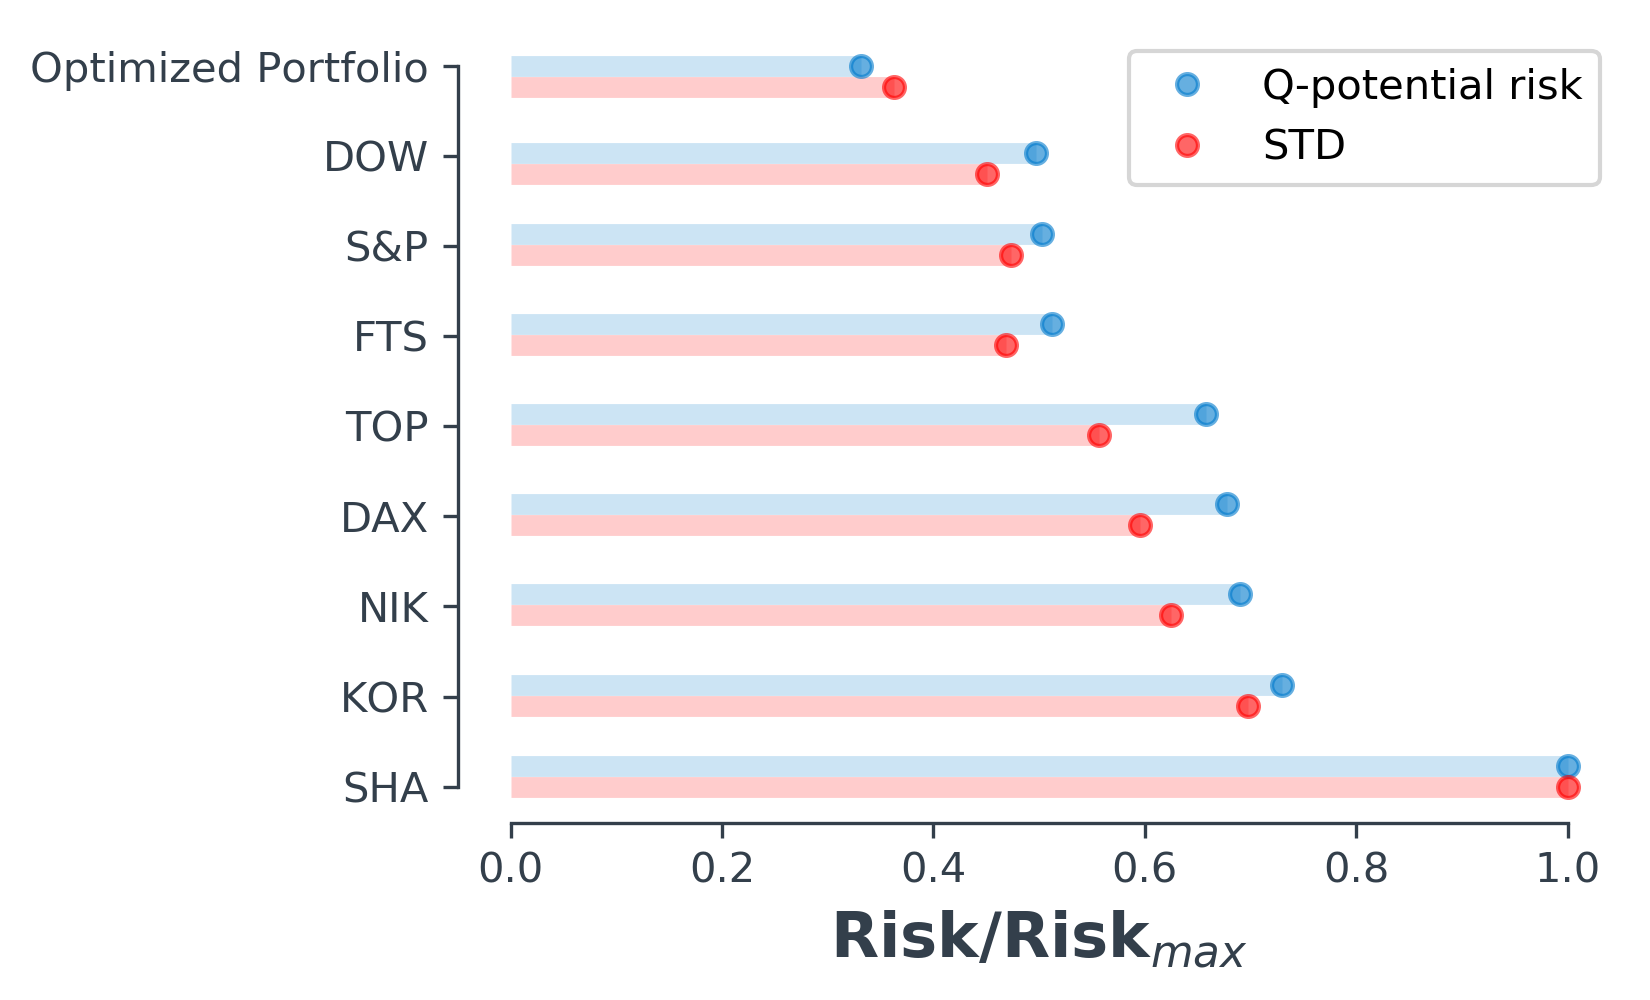
\includegraphics[width=\textwidth]{/home/hossein4527/MEGA/MEGAsync/Commit/University-Projects/MSc_Thesis/plots/fig1.png}
	\caption{سری زمانی قیمت شاخص S\&P500}
	\label{fig:1}
\end{figure}
\begin{figure}[ptb]
	\centering
	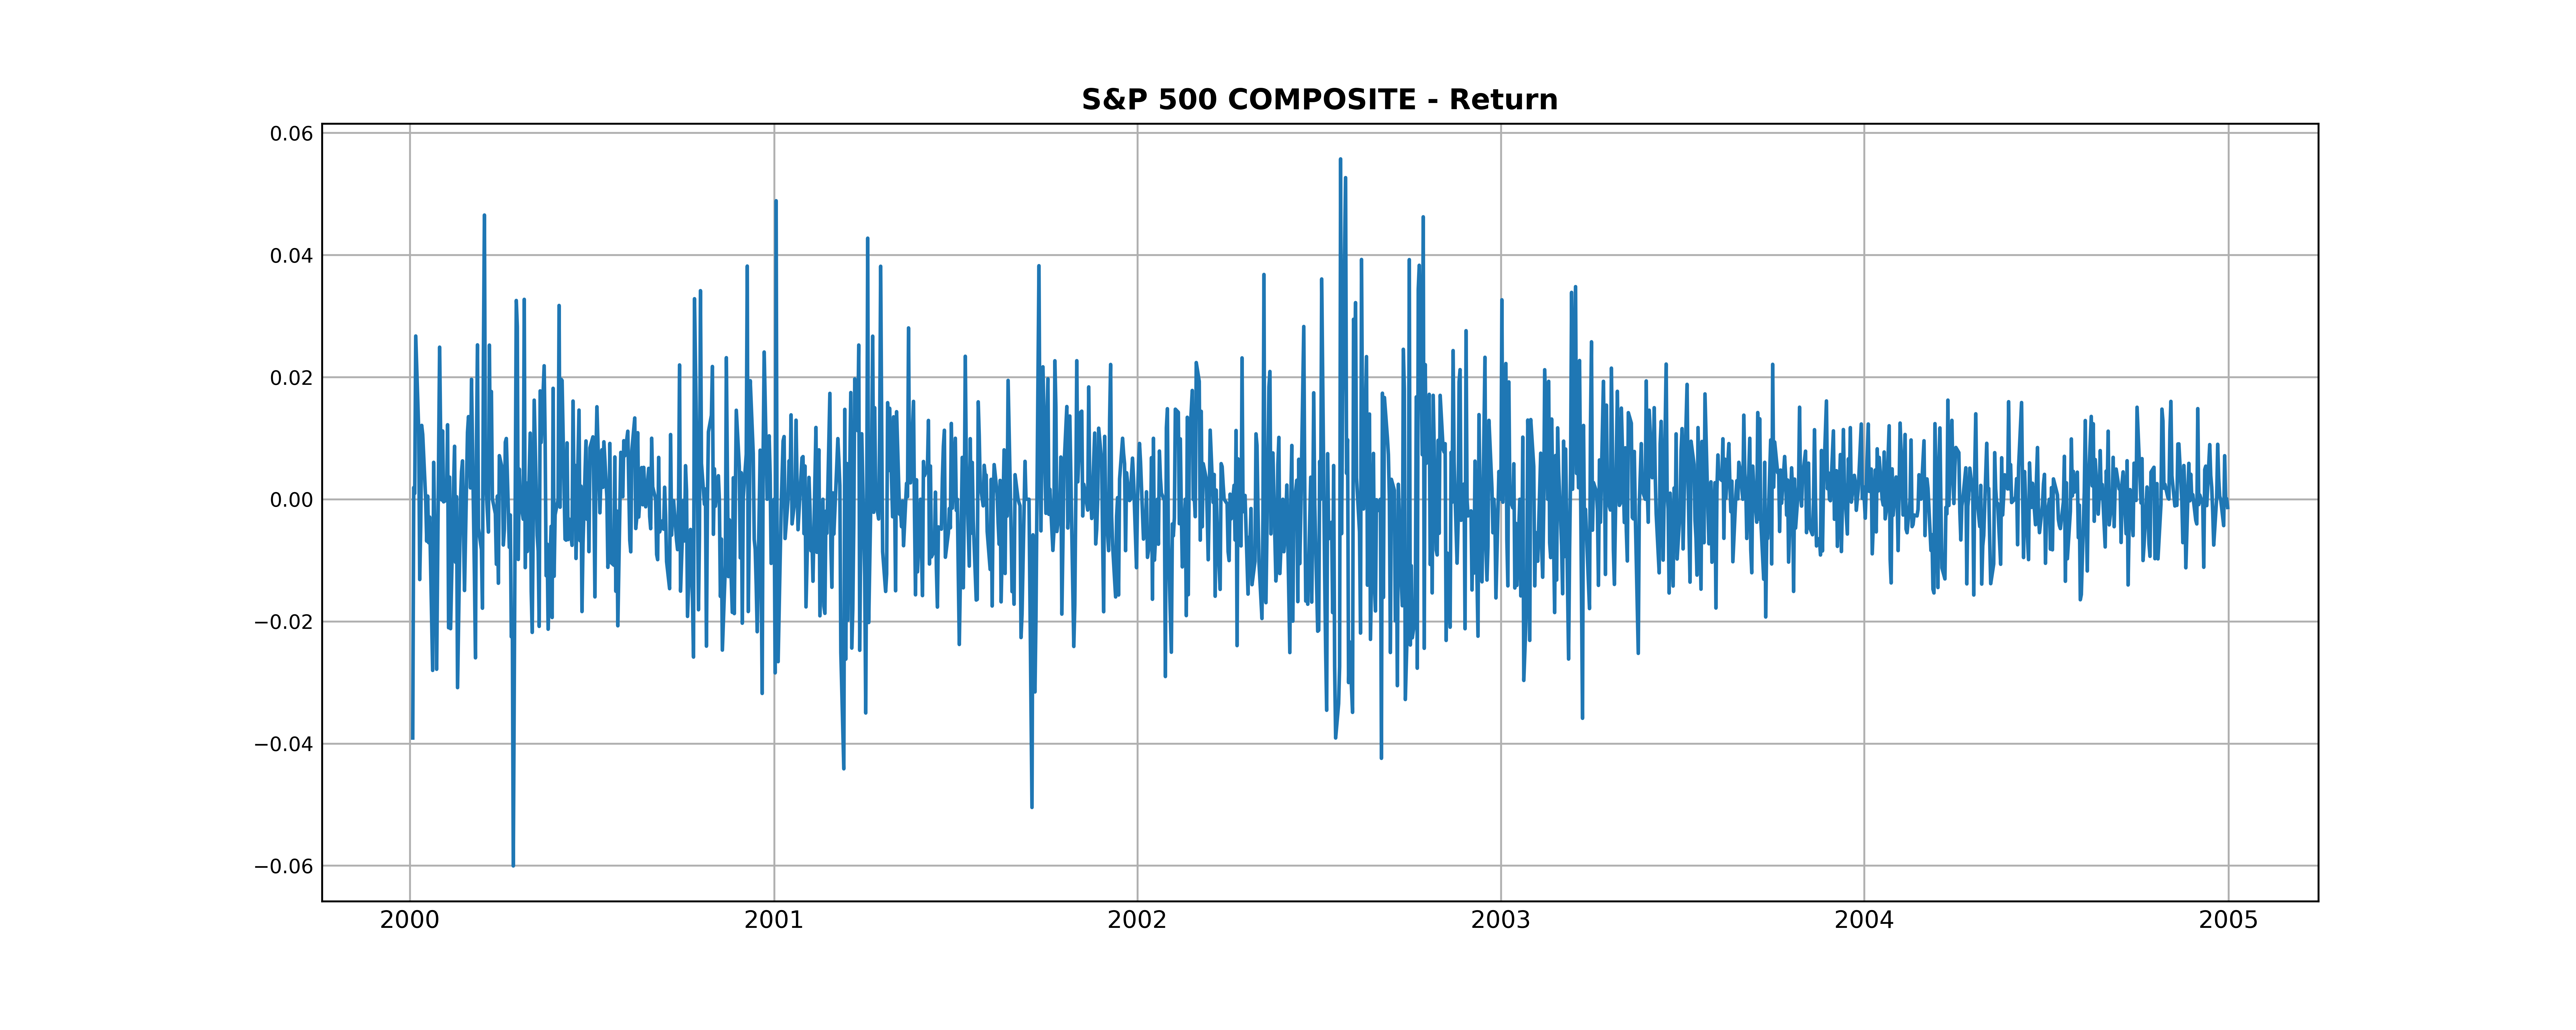
\includegraphics[width=\textwidth]{/home/hossein4527/MEGA/MEGAsync/Commit/University-Projects/MSc_Thesis/plots/fig2.png}
	\caption{سری زمانی سود شاخص S\&P500}
	\label{fig:2}
\end{figure}
با توجه به این که داده های موجود در شکل 
\ref{fig:2}
بر حسب درصد جایگذاری شده اند، خواننده های مختلف به اتفاق آرا می توانند راجع به تک تک نقاط موجود در نمودار با یک زبان صحبت کنند.
برای محاسبه پتانسیل کوانتومی حاکم بر سود و زیان بازار 
S\&P500
در بازه مشخص شده تنها یک قدم باقیست و آن هم محاسبه تابع توزیع $r(t)$، که همان پارامتر $R$ موجود در معادله 
\ref{eq:3.2}
است. برای محاسبه این پارامتر از کتابخوانه سای پای موجود در زبان پایتون کمک میگیریم. اگر برای داده های سود موجود در شکل 
\ref{fig:2}
تابع توزیع رسم کنیم به شکل
\ref{fig:3}
میرسیم.
\begin{figure}[ptb]
	\centering
	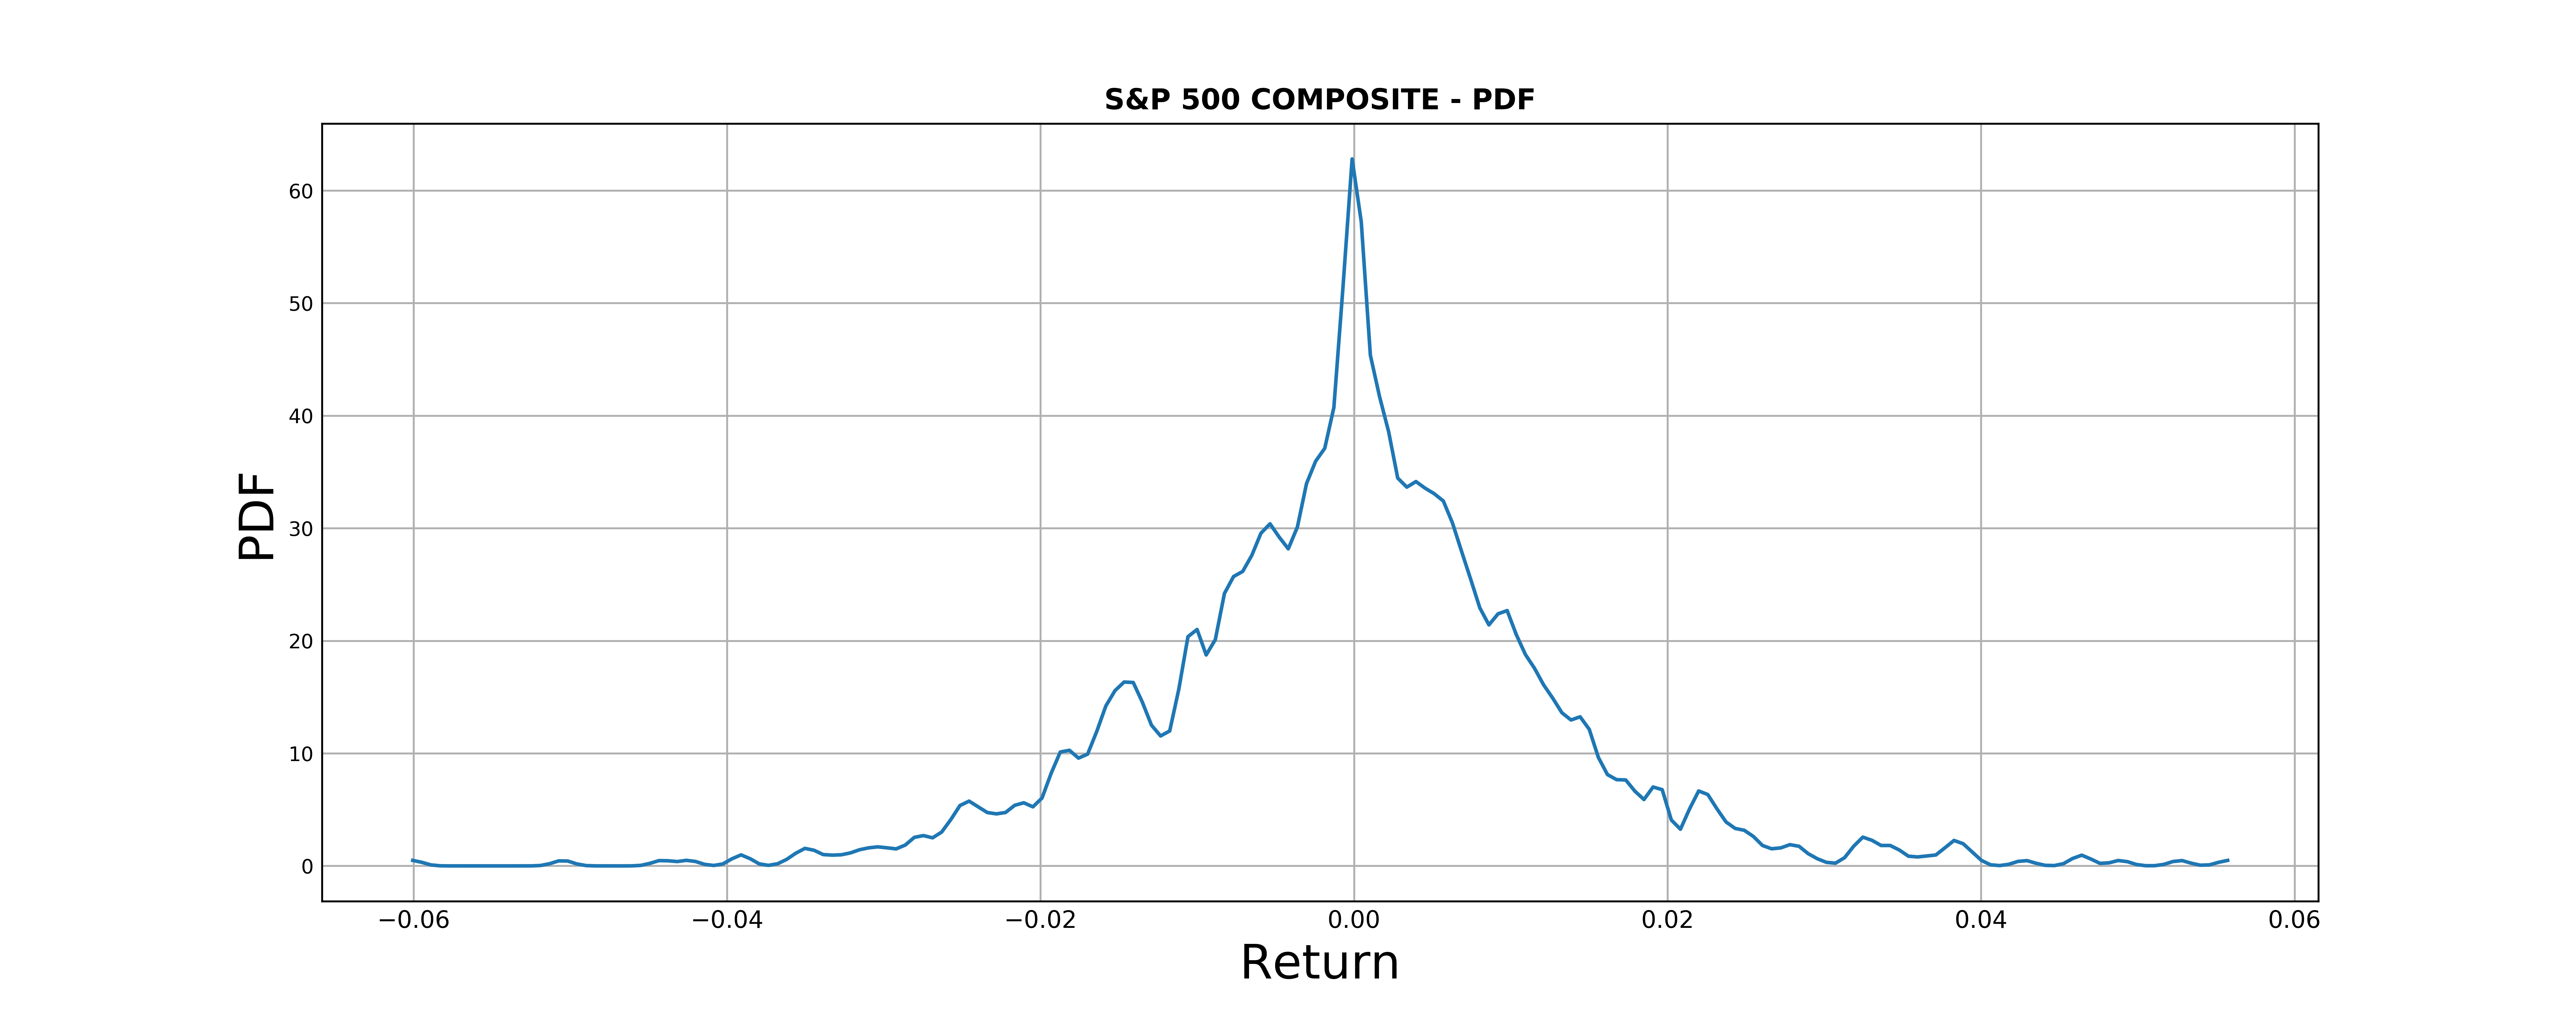
\includegraphics[width=\textwidth]{/home/hossein4527/MEGA/MEGAsync/Commit/University-Projects/MSc_Thesis/plots/fig3.png}
	\caption{تابع توزیع احتمال سود شاخص S\&P500}
	\label{fig:3}
\end{figure}
\newpage
اینک با داشتن پارامتر $R$ می توان برای محاسبه پتانسیل کوانتومی $Q$ اقدام کرد.  در مسیر این محاسبه تنها کافیست از داده های مربوط به تابع توزیع متتغیر $r$ دوبار نسبت به $r$ مشتق بگیریم و نتیجه نهایی را بر خود تابع توزیع، $R$، تقسیم کنیم. برای این کار از کتابخوانه های سای پای و نام پای موجود در زبان برنامه نویسی پایتون کمک میگیریم. شکل
\ref{fig:4}
رفتار پتانسیل کوانتومی حاکم بر بازار 
$S\&P500$
را برای بازه ۵ ساله بین سال های ۲۰۰۰ تا ۲۰۰۵ نشان می دهد. همانطور که در 
\ref{fig:4}
پیداست محور افقی بیانگر میزان سود بازار
$S\&P500$
و محور عمودی بیانگر اندازه ی پتانسیل کوانتومی حاکم بر این بازار در مقادیر مختلف مورد نظر سود است. خواننده با دید اول شهودی نسبت به حضور دو دیواره ی پتانسیلی بزرگ در انتهای مقادیر مثبت و منفی سود پیدا خواهد کرد. حضور این دو دیواره حاکی از آن است که نیرویی درست مشابه نیروی پتانسیل کوانتومی در مکانیک بوهمی در این بازه ۵ ساله از تخطی های سود و زیان بازار 
$S\&P500$
از مقادیری خاص ممانعت می کند. این مقادیر در شکل با علامت قرمز مشخص شده و همان جاییست که مقدار پتانسیل بسیار بزرگ تر از دیگر مقادیر خود است.

\begin{figure}[ptb]
	\centering
	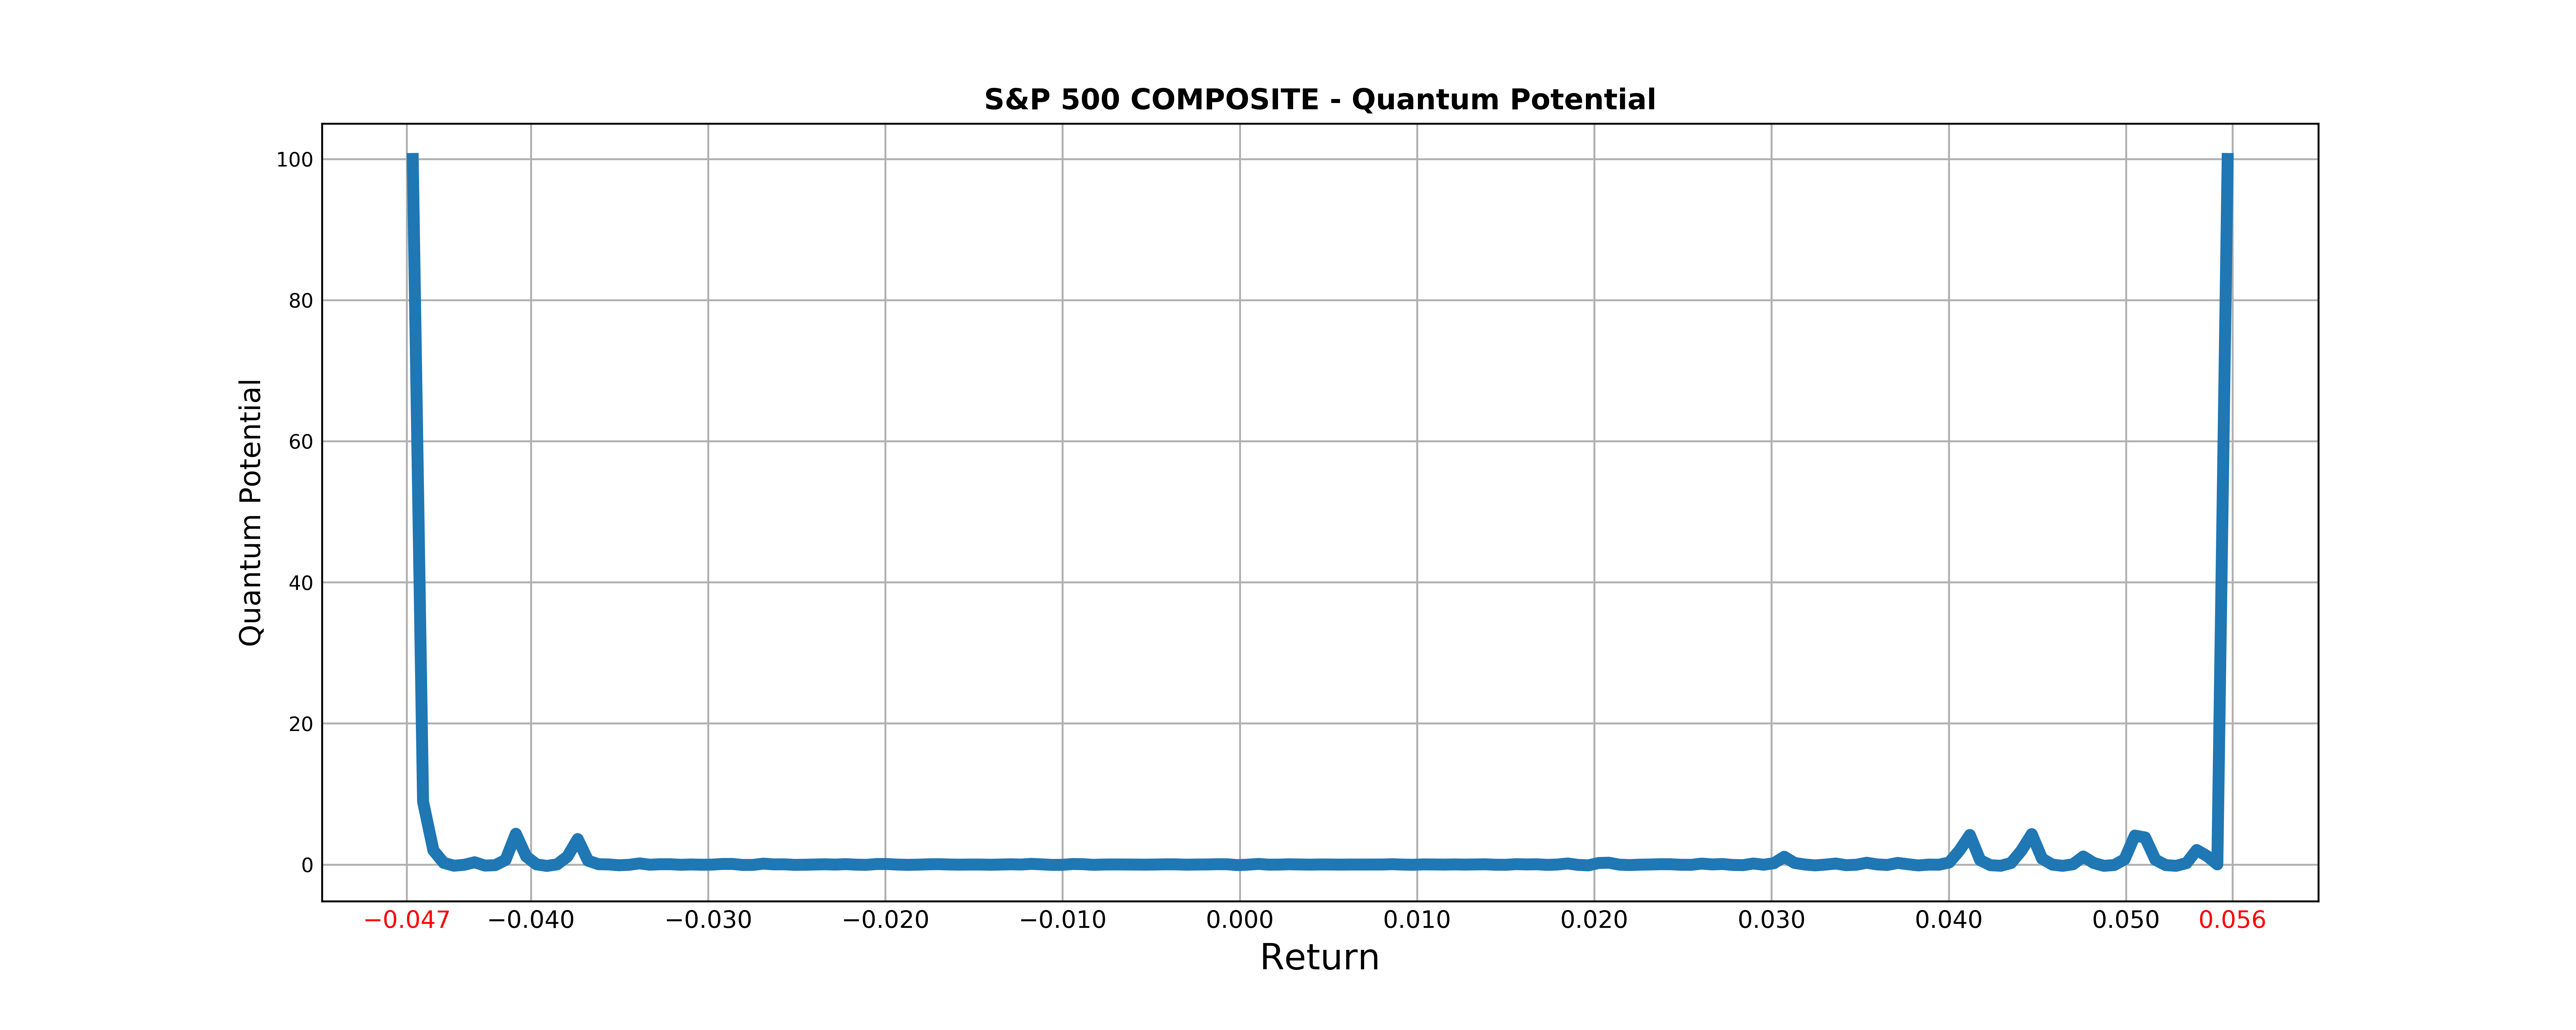
\includegraphics[width=\textwidth]{/home/hossein4527/MEGA/MEGAsync/Commit/University-Projects/MSc_Thesis/plots/fig4.png}
	\caption{تابع توزیع احتمال سود شاخص S\&P500}
	\label{fig:4}
\end{figure}
%==============================================================================================================================================================================================================================================================================================================================================================================================================================================
\chapter{مدیریت ریسک و  سبد سهام با استفاده از پتانسیل کوانتومی}


%==============================================================================================================================================================================================================================================================================================================================================================================================================================================


\chapter{خلاصه و نتیجه‌گیری}

%######################################################################################################################################################################################################################################################################################################
\begin{thebibliography}{99}

\begin{LTRitems}
	\bibitem{black}
	Black, Fischer, and Myron Scholes. "The pricing of options and corporate liabilities." Journal of political economy 81.3 (1973): 637-654.
\end{LTRitems}	
	
\begin{LTRitems}
\bibitem{bac}
Bachelier, L. (1900). Théorie de la spéculation. Annales scientifiques de l’Ecole
Normale Supérieure, 21–86.
\end{LTRitems}

\begin{LTRitems}
	\bibitem{mandel}
	Mandelbrot, Benoit B. "The variation of certain speculative prices." Fractals and scaling in finance. Springer, New York, NY, 1997. 371-418.
\end{LTRitems}

\begin{LTRitems}
	\bibitem{kada}
	Kadanoff, Leo P. "From simulation model to public policy: An examination of Forrester's" Urban Dynamics"." Simulation 16.6 (1971): 261-268.
\end{LTRitems}

\begin{LTRitems}
	\bibitem{mont}
	Montroll, Elliott W., and Wade W. Badger. Introduction to quantitative aspects of social phenomena. Gordon and Breach, 1974.
\end{LTRitems}

\begin{LTRitems}
	\bibitem{santa}
	Anderson, P. W., and K. J. Arrow. "D. Pines (eds.)(1988), The Economy as an Evolving Complex System, Redwood City."
\end{LTRitems}

\begin{LTRitems}
	\bibitem{penrose}
	Penrose, Roger. Shadows of the Mind. Vol. 4. Oxford: Oxford University Press, 1994.
\end{LTRitems}

\begin{LTRitems}
	\bibitem{hamrof}
	Hameroff, Stuart R. "Quantum coherence in microtubules: A neural basis for emergent consciousness?." Journal of consciousness studies 1.1 (1994): 91-118.
\end{LTRitems}

\begin{LTRitems}
	\bibitem{kh2}
	Khrennivov, Andrei. "Classical and quantum mechanics on information spaces with applications to cognitive, psychological, social, and anomalous phenomena." Foundations of Physics 29.7 (1999): 1065-1098.
\end{LTRitems}

\begin{LTRitems}
	\bibitem{kh3}
	Khrennikov, A. Yu. "Information Dynamics in Cognitive, Psychological." Social and Anomalous Phenomena. Kluwer (2004).
\end{LTRitems}

\begin{LTRitems}
	\bibitem{gold}
	Goldstein, Sheldon. "Bohmian mechanics and quantum information." Foundations of Physics 40.4 (2010): 335-355.
\end{LTRitems}

\begin{LTRitems}
	\bibitem{boosem}
	Bouwmeester, Dirk, and Anton Zeilinger. "The physics of quantum information: basic concepts." The physics of quantum information. Springer, Berlin, Heidelberg, 2000. 1-14.
\end{LTRitems}

\begin{LTRitems}
	\bibitem{fucks}
	Fuchs, Christopher A. "Quantum mechanics as quantum information (and only a little more)." arXiv preprint quant-ph/0205039 (2002).
\end{LTRitems}

\begin{LTRitems}
	\bibitem{kh1}
	Khrennikov, A. Y. "Ubiquitous Quantum Structure from Psychology to Finance. Springer." (2010).
\end{LTRitems}

\begin{LTRitems}
	\bibitem{haven1}
	Shen, C., and E. Haven. "Using empirical data to estimate potential functions in commodity markets: some initial results." International Journal of Theoretical Physics 56.12 (2017): 4092-4104.
\end{LTRitems}

\begin{LTRitems}
	\bibitem{tahmaseb}
	Tahmasebi, F., et al. "Financial market images: a practical approach owing to the secret quantum potential." EPL (Europhysics Letters) 109.3 (2015): 30001.
\end{LTRitems}

\begin{LTRitems}
	\bibitem{nas1}
	Nasiri, Sina, Eralp Bektas, and Gholamreza Jafari. "Risk Information of Stock Market Using Quantum Potential Constraints." Emerging Trends in Banking and Finance. Springer, Cham, 2018. 132-138.
\end{LTRitems}

\begin{LTRitems}
	\bibitem{nas2}
	Nasiri, Sina, Eralp Bektas, and G. Reza Jafari. "The impact of trading volume on the stock market credibility: Bohmian quantum potential approach." Physica A: Statistical Mechanics and its Applications 512 (2018): 1104-1112.
\end{LTRitems}

\begin{LTRitems}
	\bibitem{kh4}
	Khrennikov, Andrei Y. Ubiquitous quantum structure. Springer, 2014.
\end{LTRitems}

\begin{LTRitems}
	\bibitem{olg1}
	Choustova, Olga. Pilot wave quantum model for the stock market. No. quant-ph/0109122. 2001.
\end{LTRitems}

\begin{LTRitems}
	\bibitem{olg2}
	Choustova, Olga. "Bohmian mechanics for financial processes." Journal of Modern Optics 51.6-7 (2004): 1111-1111.
\end{LTRitems}

\begin{LTRitems}
	\bibitem{olg3}
	Choustova, Olga. "Price‐Dynamics of Shares and Bohmian Mechanics: Deterministic or Stochastic Model?." AIP Conference Proceedings. Vol. 889. No. 1. American Institute of Physics, 2007.
\end{LTRitems}

\begin{LTRitems}
	\bibitem{olg4}
	Choustova, Olga. "Quantum modeling of nonlinear dynamics of stock prices: Bohmian approach." Theoretical and Mathematical Physics 152.2 (2007): 1213-1222.
\end{LTRitems}

\begin{LTRitems}
	\bibitem{olg5}
	Choustova, Olga. "Quantum model for the price dynamics: the problem of smoothness of trajectories." Journal of mathematical analysis and applications 346.1 (2008): 296-304.
\end{LTRitems}

\begin{LTRitems}
	\bibitem{olg6}
	Choustova, Olga. "Application of Bohmian mechanics to dynamics of prices of shares: Stochastic model of Bohm–Vigier from properties of price trajectories." International Journal of Theoretical Physics 47.1 (2008): 252-260.
\end{LTRitems}

\begin{LTRitems}
	\bibitem{olg7}
	Choustova, Olga. "Quantum-like Viewpoint on the Complexity and Randomness of the Financial Market." Coping with the Complexity of Economics. Springer, Milano, 2009. 53-66.
\end{LTRitems}

\begin{LTRitems}
	\bibitem{kh8}
	Khrennikov, A. Yu. "p‐adic quantum mechanics with p‐adic valued functions." Journal of mathematical physics 32.4 (1991): 932-937.
\end{LTRitems}

\begin{LTRitems}
	\bibitem{seg}
	Segal, Wiliam, and I. E. Segal. "The Black–Scholes pricing formula in the quantum context." Proceedings of the National Academy of Sciences 95.7 (1998): 4072-4075.
\end{LTRitems}

\begin{LTRitems}
	\bibitem{baq1}
	Baaquie, Belal E. Quantum finance: Path integrals and Hamiltonians for options and interest rates. Cambridge University Press, 2007.
\end{LTRitems}

\begin{LTRitems}
	\bibitem{baq2}
	Baaquie, Belal E. "Quantum mechanics and option pricing." Department of Physics, National University of Singapore, July 28 (2005).
\end{LTRitems}

\begin{LTRitems}
	\bibitem{haven2}
	Haven, Emmanuel E. "A discussion on embedding the Black–Scholes option pricing model in a quantum physics setting." Physica A: Statistical Mechanics and its Applications 304.3-4 (2002): 507-524.
\end{LTRitems}

\begin{LTRitems}
	\bibitem{haven3}
	Haven, Emmanuel. "A Black-Scholes Schrödinger option price:‘bit’versus ‘qubit’." Physica A: Statistical Mechanics and its Applications 324.1-2 (2003): 201-206.
\end{LTRitems}

\begin{LTRitems}
	\bibitem{haven4}
	Haven, Emmanuel. "The wave-equivalent of the Black–Scholes option price: an interpretation." Physica A: Statistical Mechanics and its Applications 344.1-2 (2004): 142-145.
\end{LTRitems}

\begin{LTRitems}
	\bibitem{haven5}
	Haven, Emmanuel. "Analytical solutions to the backward Kolmogorov PDE via an adiabatic approximation to the Schrödinger PDE." Journal of mathematical analysis and applications 311.2 (2005): 439-444.
\end{LTRitems}

\begin{LTRitems}
	\bibitem{haven6}
	Haven, Emmanuel. "Bohmian mechanics in a macroscopic quantum system." AIP Conference Proceedings. Vol. 810. No. 1. American Institute of Physics, 2006.
\end{LTRitems}

\begin{LTRitems}
	\bibitem{haven7}
	Khrennikov, Andrei Yu, and Emmanuel Haven. "Quantum mechanics and violations of the sure-thing principle: The use of probability interference and other concepts." Journal of Mathematical Psychology 53.5 (2009): 378-388.
\end{LTRitems}

\begin{LTRitems}
	\bibitem{pit1}
	Piotrowski, Edward W., and Jan Sładkowski. "Quantum-like approach to financial risk: quantum anthropic principle." arXiv preprint quant-ph/0110046 (2001).
\end{LTRitems}

\begin{LTRitems}
	\bibitem{pit2}
	Piotrowski, Edward W., and J. Sładkowski. "Quantum market games." Physica A: Statistical Mechanics and its Applications 312.1-2 (2002): 208-216.
\end{LTRitems}

\begin{LTRitems}
	\bibitem{pit3}
	Piotrowski, Edward W., Jan Sładkowski, and Jacek Syska. "Interference of quantum market strategies." Physica A: Statistical Mechanics and its Applications 318.3-4 (2003): 516-528.
\end{LTRitems}

\begin{LTRitems}
	\bibitem{pit4}
	Piotrowski, Edward W., and Jan Sładkowski. "An invitation to quantum game theory." International Journal of Theoretical Physics 42.5 (2003): 1089-1099.
\end{LTRitems}

\begin{LTRitems}
	\bibitem{pit5}
	Piotrowski, Edward W. "Fixed point theorem for simple quantum strategies in quantum market games." Physica A: Statistical Mechanics and its Applications 324.1-2 (2003): 196-200.
\end{LTRitems}

\begin{LTRitems}
	\bibitem{pit6}
	Piotrowski 3, Edward W., and Jan Sładkowski. "Quantum games in finance." Quantitative Finance 4.6 (2004): 61-67.
\end{LTRitems}

\begin{LTRitems}
	\bibitem{pit7}
	Piotrowski, Edward W., Małgorzata Schroeder, and Anna Zambrzycka. "Quantum extension of European option pricing based on the Ornstein–Uhlenbeck process." Physica A: Statistical Mechanics and its Applications 368.1 (2006): 176-182.
\end{LTRitems}

\begin{LTRitems}
	\bibitem{geg}
	Granger, C. W. "Is chaotic economic theory relevant for economics? A review essay." Journal of International and Comparative Economics 3 (1994): 139-145.
\end{LTRitems}

\begin{LTRitems}
	\bibitem{geg1}
	Barnett, William A., and Apostolos Serletis. "Martingales, nonlinearity, and chaos." Journal of Economic Dynamics and Control 24.5-7 (2000): 703-724.
\end{LTRitems}

\begin{LTRitems}
	\bibitem{geg2}
	Benhabib, Jess, ed. Cycles and chaos in economic equilibrium. Princeton University Press, 1992.
\end{LTRitems}

\begin{LTRitems}
	\bibitem{geg3}
	Brock, William A., and Chera L. Sayers. "Is the business cycle characterized by deterministic chaos?." Journal of monetary economics 22.1 (1988): 71-90.
\end{LTRitems}

\begin{LTRitems}
	\bibitem{geg4}
	Campbell, John Y., et al. The econometrics of financial markets. princeton University press, 1997.
\end{LTRitems}

\begin{LTRitems}
	\bibitem{geg5}
	Hsieh, David A. "Chaos and nonlinear dynamics: application to financial markets." The journal of finance 46.5 (1991): 1839-1877.
\end{LTRitems}

\begin{LTRitems}
	\bibitem{sam1}
	Samuelson, Paul A. "Proof that properly anticipated prices fluctuate randomly." The world scientific handbook of futures markets. 2016. 25-38.
\end{LTRitems}

\begin{LTRitems}
	\bibitem{sam2}
	Samuelson, Paul A. "Rational theory of warrant pricing." Henry P. McKean Jr. Selecta. Birkhäuser, Cham, 2015. 195-232.
\end{LTRitems}

\begin{LTRitems}
	\bibitem{fama}
	Malkiel, Burton G., and Eugene F. Fama. "Efficient capital markets: A review of theory and empirical work." The journal of Finance 25.2 (1970): 383-417.
\end{LTRitems}

\begin{LTRitems}
	\bibitem{stan}
	Stanley, H. Eugene, and Rosario N. Mantegna. An introduction to econophysics. Cambridge University Press, Cambridge, 2000.
\end{LTRitems}

\begin{LTRitems}
	\bibitem{shia}
	Shiryaev, Albert N. Essentials of stochastic finance: facts, models, theory. Vol. 3. World scientific, 1999.
\end{LTRitems}

\begin{LTRitems}
	\bibitem{bohm1}
	Bohm, D., B. J. Hiley, and P. Holland. "Book-Review-the Undivided Universe-an Ontological Interpretation of Quantum Theory." Nature 366 (1993): 420.	
\end{LTRitems}

\begin{LTRitems}
	\bibitem{bohm2}
	Hiley, Basil, and P. Pylkkänen. "Active information and cognitive science–A reply to Kieseppä." Brain, mind and physics (1997): 64-85.
\end{LTRitems}


\begin{LTRitems}
	\bibitem{shen}
	Shen, C., and E. Haven. "Using empirical data to estimate potential functions in commodity markets: some initial results." International Journal of Theoretical Physics 56.12 (2017): 4092-4104.
\end{LTRitems}

\begin{LTRitems}
	\bibitem{}
	
\end{LTRitems}

\begin{LTRitems}
	\bibitem{}
	
\end{LTRitems}

\begin{LTRitems}
	\bibitem{}
	
\end{LTRitems}

\begin{LTRitems}
	\bibitem{}
	
\end{LTRitems}

\begin{LTRitems}
	\bibitem{}
	
\end{LTRitems}

\begin{LTRitems}
	\bibitem{}
	
\end{LTRitems}



\end{thebibliography}

\end{document}
